\documentclass[11pt]{article}
\usepackage[utf8]{inputenc}

% Increase main memory size
\usepackage{etex}
\usepackage{morewrites}
\usepackage{multicol}
\usepackage{pgfplots}
\usepackage{tikz}
\usetikzlibrary{external}
\tikzexternalize[prefix=cached_models/]
% Ensure the directory exists
\immediate\write18{mkdir -p cached_models}

\usepackage{etex}
\usepackage{morewrites}
\usepackage{enumitem}
\usepackage{float}

\listfiles

\usepackage{amsmath, amssymb, amsthm}
\usepackage{graphicx}
\usepackage{geometry}
\usepackage{array}
\usepackage{booktabs}
\usepackage{float}
\usepackage{verbatim}
\usetikzlibrary{3d}

% Page Layout
\geometry{a4paper, margin=1in}
\setlength\parindent{0pt}
\pgfplotsset{compat=1.18}

% Custom commands
\newcommand{\card}[1]{\lvert #1 \rvert}
\newcommand{\inner}[2]{\left\langle #1, #2 \right\rangle}

\title{\textbf{Principles of Mathematical Analysis}}
\author{}
\date{}

\begin{document}

\maketitle

\section{Measure Theory}
\subsection{Riemann Integral}
For a bounded function \( f: [a, b] \to \mathbb{R} \) and any partition of the interval \([a, b]\), \(P = \{a = x_0 < x_1 < \ldots < x_n = b\}\), we consider on each subinterval \(I_j = [x_{j-1}, x_j], \quad j = 1, \ldots, n\), the quantities:
\[M_j = \sup_{x \in I_j} f(x), \quad m_j = \inf_{x \in I_j} f(x).\]

We also define the upper and lower sums of \(f\) with respect to the partition \(P\) as:
\[U_f(P) = \sum_{j=1}^{n} M_j (x_j - x_{j-1}), \quad L_f(P) = \sum_{j=1}^{n} m_j (x_j - x_{j-1}).\]

\begin{center}
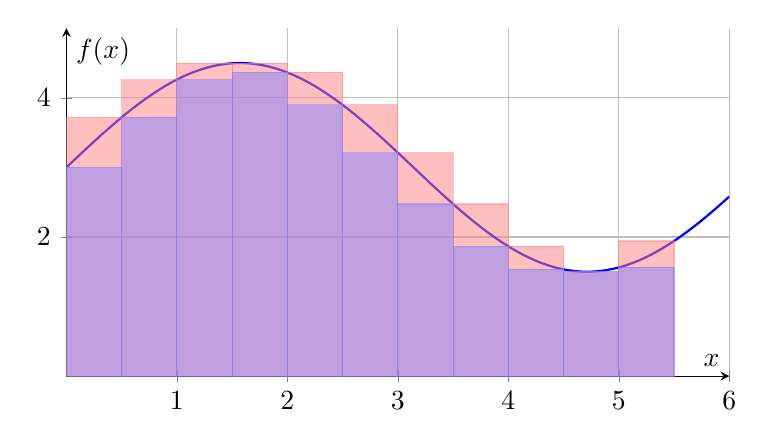
\begin{tikzpicture}
    \begin{axis}[
        axis lines = middle,
        xlabel = \(x\),
        ylabel = {\(f(x)\)},
        domain=0:6,
        samples=100,
        ymin=0, ymax=5,
        xmin=0, xmax=6,
        width=10cm,
        height=6cm,
        grid=both,
    ]
    \addplot[blue, thick] {1.5*sin(deg(x)) + 3};
    \addplot[red!50, fill=red!50, opacity=0.5] coordinates {(0,0) (0,{1.5*sin(deg(0.5))+3}) (0.5,{1.5*sin(deg(0.5))+3}) (0.5,0)} -- cycle;
    \addplot[red!50, fill=red!50, opacity=0.5] coordinates {(0.5,0) (0.5,{1.5*sin(deg(1))+3}) (1,{1.5*sin(deg(1))+3}) (1,0)} -- cycle;
    \addplot[red!50, fill=red!50, opacity=0.5] coordinates {(1,0) (1,{1.5*sin(deg(1.5))+3}) (1.5,{1.5*sin(deg(1.5))+3}) (1.5,0)} -- cycle;
    \addplot[red!50, fill=red!50, opacity=0.5] coordinates {(1.5,0) (1.5,{1.5*sin(deg(1.5))+3}) (2,{1.5*sin(deg(1.5))+3}) (2,0)} -- cycle;
    \addplot[red!50, fill=red!50, opacity=0.5] coordinates {(2,0) (2,{1.5*sin(deg(2))+3}) (2.5,{1.5*sin(deg(2))+3}) (2.5,0)} -- cycle;
    \addplot[red!50, fill=red!50, opacity=0.5] coordinates {(2.5,0) (2.5,{1.5*sin(deg(2.5))+3}) (3,{1.5*sin(deg(2.5))+3}) (3,0)} -- cycle;
    \addplot[red!50, fill=red!50, opacity=0.5] coordinates {(3,0) (3,{1.5*sin(deg(3))+3}) (3.5,{1.5*sin(deg(3))+3}) (3.5,0)} -- cycle;
    \addplot[red!50, fill=red!50, opacity=0.5] coordinates {(3.5,0) (3.5,{1.5*sin(deg(3.5))+3}) (4,{1.5*sin(deg(3.5))+3}) (4,0)} -- cycle;
    \addplot[red!50, fill=red!50, opacity=0.5] coordinates {(4,0) (4,{1.5*sin(deg(4))+3}) (4.5,{1.5*sin(deg(4))+3}) (4.5,0)} -- cycle;
    \addplot[red!50, fill=red!50, opacity=0.5] coordinates {(4.5,0) (4.5,{1.5*sin(deg(4.66))+3}) (5,{1.5*sin(deg(4.66))+3}) (5,0)} -- cycle;
    \addplot[red!50, fill=red!50, opacity=0.5] coordinates {(5,0) (5,{1.5*sin(deg(5.5))+3}) (5.5,{1.5*sin(deg(5.5))+3}) (5.5,0)} -- cycle;

    \addplot[blue!50, fill=blue!50, opacity=0.5] coordinates {(0,0) (0,{1.5*sin(deg(0))+3}) (0.5,{1.5*sin(deg(0))+3}) (0.5,0)} -- cycle;
    \addplot[blue!50, fill=blue!50, opacity=0.5] coordinates {(0.5,0) (0.5,{1.5*sin(deg(0.5))+3}) (1,{1.5*sin(deg(0.5))+3}) (1,0)} -- cycle;
    \addplot[blue!50, fill=blue!50, opacity=0.5] coordinates {(1,0) (1,{1.5*sin(deg(1))+3}) (1.5,{1.5*sin(deg(1))+3}) (1.5,0)} -- cycle;
    \addplot[blue!50, fill=blue!50, opacity=0.5] coordinates {(1.5,0) (1.5,{1.5*sin(deg(2))+3}) (2,{1.5*sin(deg(2))+3}) (2,0)} -- cycle;
    \addplot[blue!50, fill=blue!50, opacity=0.5] coordinates {(2,0) (2,{1.5*sin(deg(2.5))+3}) (2.5,{1.5*sin(deg(2.5))+3}) (2.5,0)} -- cycle;
    \addplot[blue!50, fill=blue!50, opacity=0.5] coordinates {(2.5,0) (2.5,{1.5*sin(deg(3))+3}) (3,{1.5*sin(deg(3))+3}) (3,0)} -- cycle;
    \addplot[blue!50, fill=blue!50, opacity=0.5] coordinates {(3,0) (3,{1.5*sin(deg(3.5))+3}) (3.5,{1.5*sin(deg(3.5))+3}) (3.5,0)} -- cycle;
    \addplot[blue!50, fill=blue!50, opacity=0.5] coordinates {(3.5,0) (3.5,{1.5*sin(deg(4))+3}) (4,{1.5*sin(deg(4))+3}) (4,0)} -- cycle;
    \addplot[blue!50, fill=blue!50, opacity=0.5] coordinates {(4,0) (4,{1.5*sin(deg(4.5))+3}) (4.5,{1.5*sin(deg(4.5))+3}) (4.5,0)} -- cycle;
    \addplot[blue!50, fill=blue!50, opacity=0.5] coordinates {(4.5,0) (4.5,{1.5*sin(deg(4.66))+3}) (5,{1.5*sin(deg(4.66))+3}) (5,0)} -- cycle;
    \addplot[blue!50, fill=blue!50, opacity=0.5] coordinates {(5,0) (5,{1.5*sin(deg(5))+3}) (5.5,{1.5*sin(deg(5))+3}) (5.5,0)} -- cycle;
    \end{axis}
\end{tikzpicture}
\end{center}

For any two partitions \(P\) and \(Q\) of \([a, b]\), we have:
\[L_f(P) \leq \text{Area under } f \leq U_f(Q).\]

If $P$ has a value $I$ such that:
\[\sup_{P} L_f(P) = I = \inf_{P} U_f(P),\]
then we say that \(f\) is Riemann integrable on \([a, b]\) and define the Riemann integral of \(f\) over \([a, b]\) as:
\[\int_a^b f(x) \, dx = I.\]

Continuous functions on closed intervals are Riemann integrable.
\subsection{The Lebesgue Integral}
A bounded function \( f: [a, b] \to \mathbb{R} \) is said to be \textit{Lebesgue integrable} on \([a, b]\) if the set of points where \(f\) is discontinuous has zero measure. 

A set $B \subset \mathbb{R}$ has \textit{measure zero} if for every $\varepsilon > 0$, it can be covered by a countable collection of open intervals $\{(a_n, b_n)\}$ such that:
\[B \subset \bigcup_{n=1}^{\infty} (a_n, b_n) \quad \text{and} \quad \sum_{n=1}^{\infty} (b_n - a_n) < \varepsilon.\]

\subsubsection{Example: Dirichlet Function}
The Dirichlet function:
\[ f(x) = \chi_{\mathbb{Q}}(x) = \begin{cases} 1 & \text{if } x \in \mathbb{Q}, \\ 0 & \text{if } x \notin \mathbb{Q}, \end{cases} \]

On the interval \([0, 1]\): 
\begin{center}
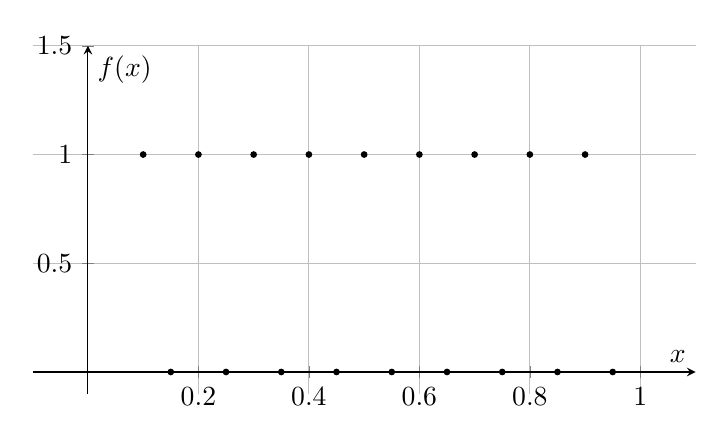
\begin{tikzpicture}
    \begin{axis}[
        axis lines = middle,
        xlabel = \(x\),
        ylabel = {\(f(x)\)},
        domain=0:1,
        samples=100,
        ymin=-0.1, ymax=1.5,
        xmin=-0.1, xmax=1.1,
        width=10cm,
        height=6cm,
        grid=both,
    ]
    \addplot[only marks, mark=*, mark size=1pt] coordinates {
        (0.1,1) (0.2,1) (0.3,1) (0.4,1) (0.5,1) (0.6,1) (0.7,1) (0.8,1) (0.9,1)
        (0.15,0) (0.25,0) (0.35,0) (0.45,0) (0.55,0) (0.65,0) (0.75,0) (0.85,0) (0.95,0)
    };
    \end{axis}
\end{tikzpicture}
\end{center}

We see that \(f\) is not Riemann integrable since it is discontinuous everywhere. 

But consider, 
\[\mathbb{Q} = \{q_1, q_2, q_3, \ldots\}\] 
and define:
\[f_1(x) = \chi_{\{q_1\}}(x) \rightarrow \text{integrable on } [0, 1]\]
\[f_2(x) = \chi_{\{q_1, q_2\}}(x) \rightarrow \text{integrable on } [0, 1]\]
\[\vdots\]
\[f_n(x) = \chi_{\{q_1, q_2, \ldots, q_n\}}(x) \rightarrow \text{integrable on } [0, 1]\]

Then,
\[\lim_{n \to \infty} f_n(x) = \chi_{\mathbb{Q}}(x).\]

\subsubsection{Characteristic Function}
For any set \(A \subset \mathbb{R}\), the characteristic function \(\chi_A: \mathbb{R} \to \{0, 1\}\) is defined as:
\[\chi_A(x) = \begin{cases} 1 & \text{if } x \in A, \\ 0 & \text{if } x \notin A. \end{cases}\]

\[\int_0^1 f_1(x) \, dx = 0 = \int_0^1 f_2(x) \, dx = \ldots = \int_0^1 f_n(x) \, dx = 0.\]

\subsubsection*{Example}
Let 
\[f_n(x) = \begin{cases} x^n & \text{if } 0 \leq x < 1, \\ 0 & \text{if } 1 \leq x. \end{cases}\]

Then, with $f_n(x)$ continuous on $\mathbb{R}$, we have:
\[\lim_{n \to \infty} f_n(x) = \begin{cases} 1 & \text{if } 0 \leq x < 1, \\ 0 & \text{if } 1 \leq x. \end{cases}\]
so we can see that there is a discontinuity at \(x = 1\).

\begin{center}
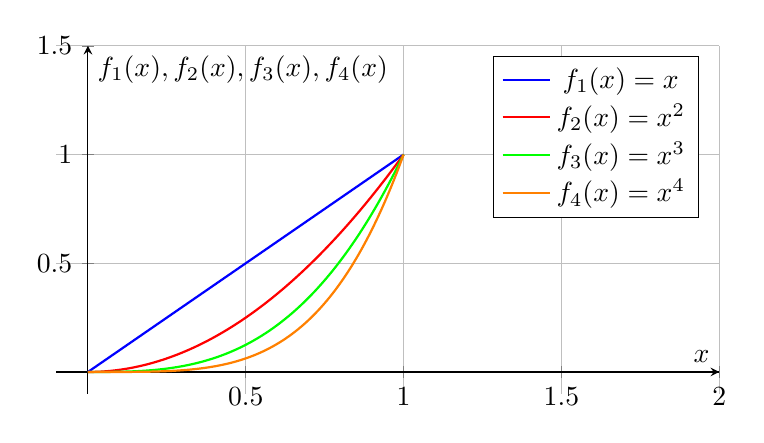
\begin{tikzpicture}
    \begin{axis}[
        axis lines = middle,
        xlabel = \(x\),
        ylabel = {\(f_1(x), f_2(x), f_3(x), f_4(x)\)},
        domain=0:1,
        samples=100,
        ymin=-0.1, ymax=1.5,
        xmin=-0.1, xmax=2,
        width=10cm,
        height=6cm,
        grid=both,
        legend pos=north east
    ]
    \addplot[blue, thick] {x};
    \addlegendentry{\(f_1(x) = x\)}

    \addplot[red, thick] {x^2};
    \addlegendentry{\(f_2(x) = x^2\)}

    \addplot[green, thick] {x^3};
    \addlegendentry{\(f_3(x) = x^3\)}

    \addplot[orange, thick] {x^4};
    \addlegendentry{\(f_4(x) = x^4\)}

    \addplot[black, thick] coordinates {(1,0) (2,0)};
    \end{axis}
\end{tikzpicture}
\end{center}

\subsubsection*{Example}
Let
\[f_n(x) = \begin{cases} -1 & \text{if } x \leq -\frac{1}{n}, \\ \sin\left(\dfrac{n\pi x}{2}\right) & \text{if } -\frac{1}{n} \leq x \leq \frac{1}{n}, \\ 1 & \text{if } \frac{1}{n} \leq x. \end{cases}\]

Then, with $f_n(x)$ continuous and differentiable on $\mathbb{R}$, we have:
\[\lim_{n \to \infty} f_n(x) = \begin{cases} -1 & \text{if } x < 0, \\ 0 & \text{if } x = 0, \\ 1 & \text{if } x > 0. \end{cases}\]
\begin{center}
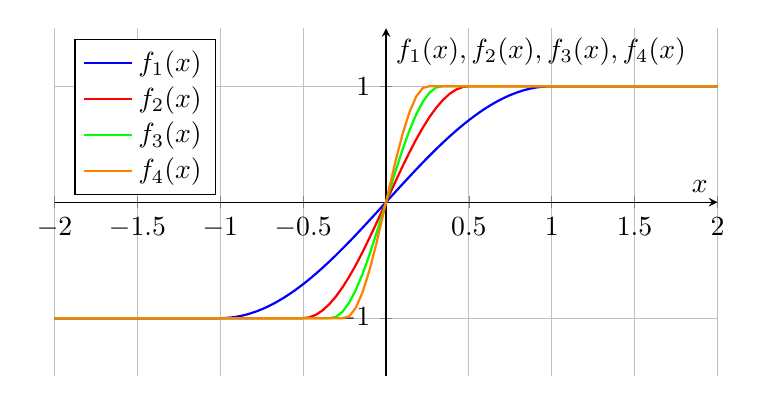
\begin{tikzpicture}
    \begin{axis}[
        axis lines = middle,
        xlabel = \(x\),
        ylabel = {\(f_1(x), f_2(x), f_3(x), f_4(x)\)},
        domain=-2:2,
        samples=100,
        ymin=-1.5, ymax=1.5,
        xmin=-2, xmax=2,
        width=10cm,
        height=6cm,
        grid=both,
        legend pos=north west
    ]
    \addplot[blue, thick] {x <= -1 ? -1 : (x >= 1 ? 1 : sin(deg(pi*x/2)))};
    \addlegendentry{\(f_1(x)\)}

    \addplot[red, thick] {x <= -0.5 ? -1 : (x >= 0.5 ? 1 : sin(deg(2*pi*x/2)))};
    \addlegendentry{\(f_2(x)\)}

    \addplot[green, thick] {x <= -0.33 ? -1 : (x >= 0.33 ? 1 : sin(deg(3*pi*x/2)))};
    \addlegendentry{\(f_3(x)\)}

    \addplot[orange, thick] {x <= -0.25 ? -1 : (x >= 0.25 ? 1 : sin(deg(4*pi*x/2)))};
    \addlegendentry{\(f_4(x)\)}
    \end{axis}
\end{tikzpicture}
\end{center}

\subsubsection*{Example}
The Dirichlet function is not integrable but it is the limit of a sequence of integrable functions, all with integral equal to zero.

We need to define a new kind of convergence.

\subsection{Convergences}
A sequence of functions \(\{f_n\}_{n \in \mathbb{N}}\) converges punctually to a function \(f\) on \(Dom(f)\) if:
\[\lim_{n \to \infty} f_n(x) = f(x), \quad \forall x \in Dom(f).\]

A sequence of functions \(\{f_n\}_{n \in \mathbb{N}}\) converges uniformly to a function \(f\) on \(Dom(f)\) if:
\[\forall \varepsilon, \quad \exists N : n > N \implies |f_n(x) - f(x)| < \varepsilon, \quad \forall x \in Dom(f).\]

\subsubsection*{Example}
Let
\[f_n(x) = \frac{1}{n} \sin(nx), \quad x \in \mathbb{R} \stackrel{n \to \infty}{\longrightarrow} 0.\]

\begin{center}
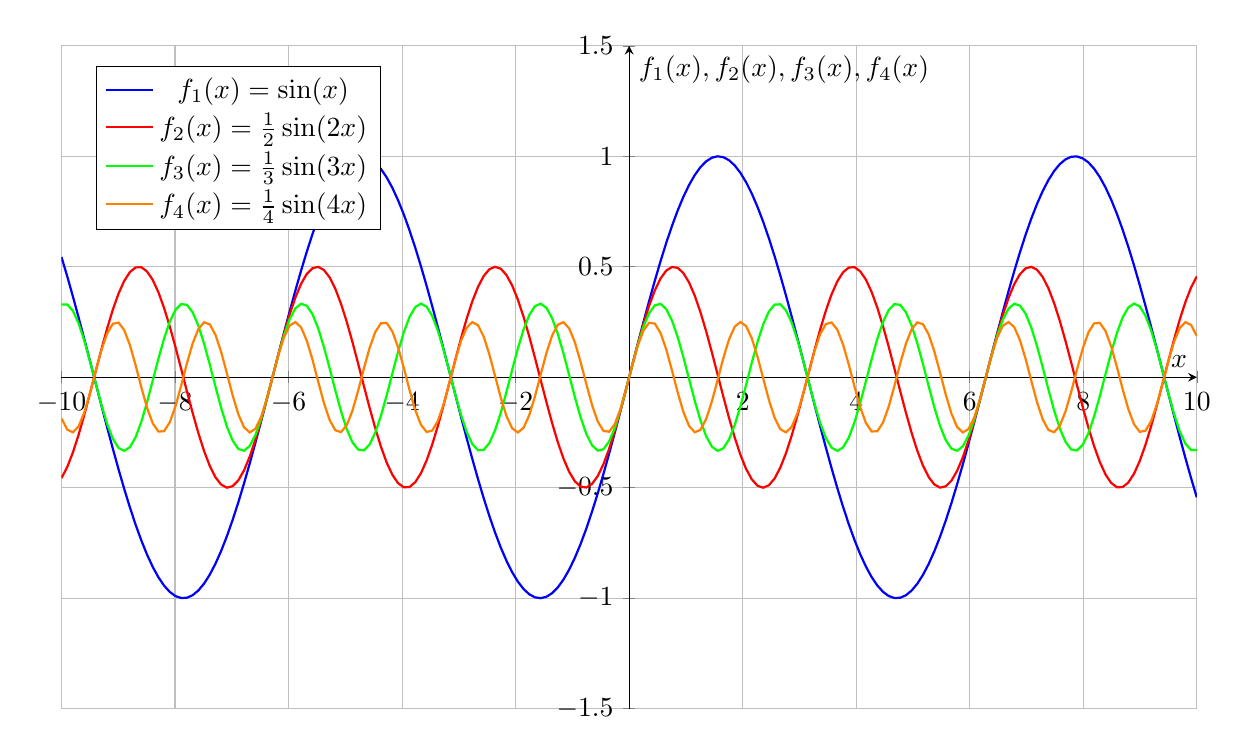
\begin{tikzpicture}
    \begin{axis}[
        axis lines = middle,
        xlabel = \(x\),
        ylabel = {\(f_1(x), f_2(x), f_3(x), f_4(x)\)},
        domain=-10:10,
        samples=200,
        ymin=-1.5, ymax=1.5,
        xmin=-10, xmax=10,
        width=16cm,
        height=10cm,
        grid=both,
        legend pos=north west
    ]
    \addplot[blue, thick] {1*sin(deg(x))};
    \addlegendentry{\(f_1(x) = \sin(x)\)}

    \addplot[red, thick] {1/2*sin(deg(2*x))};
    \addlegendentry{\(f_2(x) = \frac{1}{2}\sin(2x)\)}

    \addplot[green, thick] {1/3*sin(deg(3*x))};
    \addlegendentry{\(f_3(x) = \frac{1}{3}\sin(3x)\)}

    \addplot[orange, thick] {1/4*sin(deg(4*x))};
    \addlegendentry{\(f_4(x) = \frac{1}{4}\sin(4x)\)}
    \end{axis}
\end{tikzpicture}
\end{center}

\subsubsection{Uniform Convergence}
\begin{enumerate}
    \item If \(\{f_n\}_{n \in \mathbb{N}}\) converges uniformly to \(f\) on \([a, b]\) and each \(f_n\) is continuous, then:
        \[\int_a^b f(x) \, dx = \lim_{n \to \infty} \int_a^b f_n(x) \, dx.\]
    \item If \(\{f_n\}_{n \in \mathbb{N}}\) converges uniformly to \(f\) on \([a, b]\) and each \(f_n\) is continuous in \([a, b]\), then \(f\) is continuous on \([a, b]\).
    \item If \(\{f_n\}_{n \in \mathbb{N}}\) is a sequence of differentiable functions on \([a, b]\) that converges punctually to some continuous function \(f\) on \([a, b]\) and if the sequence of derivatives \(\{f_n'\}_{n \in \mathbb{N}}\) converges uniformly to some continuous function \(g\), then \(f\) is differentiable on \((a, b)\) and:
        \[f'(x) = g(x) = \lim_{n \to \infty} f_n'(x).\]
\end{enumerate}

\subsubsection{Henri Lebesgue (1875-1941)}
How can we count money in bills?
\begin{enumerate}
    \item Add each amount as the bills come in. (Riemann)
    \item Make groups by denomination and count each group. (Lebesgue)
\end{enumerate}

This is the idea behind the Lebesgue integral.

\subsection{Cantor Ternary Set}
\vskip 1em
\begin{center}
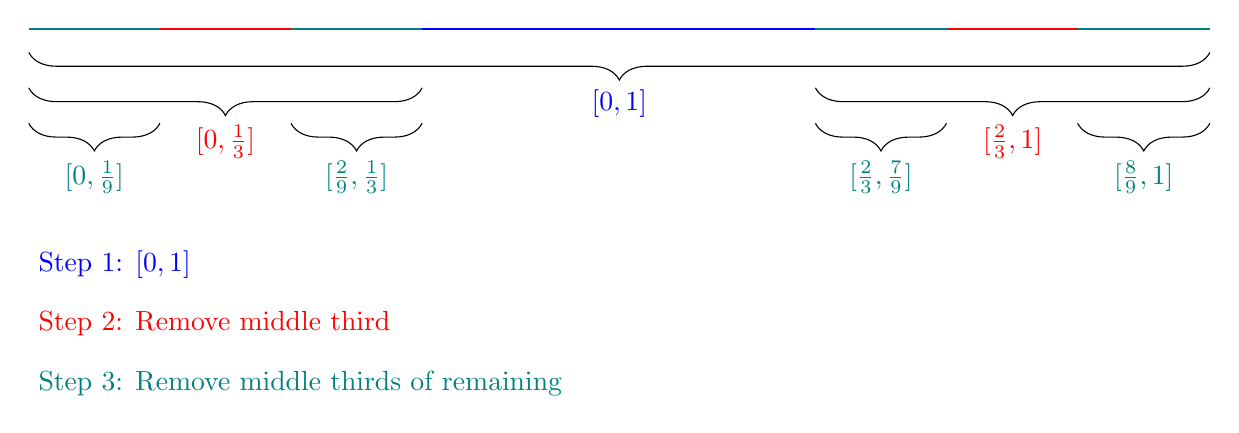
\begin{tikzpicture}[scale=1.5]
    % Step 1
    \draw[thick, blue] (0, 0) -- (10, 0);
    \draw[decorate, decoration={brace, mirror, amplitude=10pt}] (0, -0.2) -- (10, -0.2) node[midway, below=10pt] {\textcolor{blue}{\([0, 1]\)}};

    % Step 2
    \draw[thick, red] (0, 0) -- (3.33, 0);
    \draw[thick, red] (6.66, 0) -- (10, 0);
    \draw[decorate, decoration={brace, mirror, amplitude=10pt}] (0, -0.5) -- (3.33, -0.5) node[midway, below=10pt] {\textcolor{red}{\([0, \frac{1}{3}]\)}};
    \draw[decorate, decoration={brace, mirror, amplitude=10pt}] (6.66, -0.5) -- (10, -0.5) node[midway, below=10pt] {\textcolor{red}{\([\frac{2}{3}, 1]\)}};

    % Step 3
    \draw[thick, teal] (0, 0) -- (1.11, 0);
    \draw[thick, teal] (2.22, 0) -- (3.33, 0);
    \draw[thick, teal] (6.66, 0) -- (7.77, 0);
    \draw[thick, teal] (8.88, 0) -- (10, 0);
    \draw[decorate, decoration={brace, mirror, amplitude=10pt}] (0, -0.8) -- (1.11, -0.8) node[midway, below=10pt] {\textcolor{teal}{\([0, \frac{1}{9}]\)}};
    \draw[decorate, decoration={brace, mirror, amplitude=10pt}] (2.22, -0.8) -- (3.33, -0.8) node[midway, below=10pt] {\textcolor{teal}{\([\frac{2}{9}, \frac{1}{3}]\)}};
    \draw[decorate, decoration={brace, mirror, amplitude=10pt}] (6.66, -0.8) -- (7.77, -0.8) node[midway, below=10pt] {\textcolor{teal}{\([\frac{2}{3}, \frac{7}{9}]\)}};
    \draw[decorate, decoration={brace, mirror, amplitude=10pt}] (8.88, -0.8) -- (10, -0.8) node[midway, below=10pt] {\textcolor{teal}{\([\frac{8}{9}, 1]\)}};

    % Legend
    \node[anchor=west] at (0, -2) {\textcolor{blue}{Step 1: \([0, 1]\)}};
    \node[anchor=west] at (0, -2.5) {\textcolor{red}{Step 2: Remove middle third}};
    \node[anchor=west] at (0, -3) {\textcolor{teal}{Step 3: Remove middle thirds of remaining}};
\end{tikzpicture}
\end{center}

The Cantor set \(C\) is obtained by removing the open middle third of each remaining interval at each step. Then,
\[C = [0, 1] \setminus J = \bigcup_{n=1}^{\infty} J_n,\]
where \(J\) is the union of all removed intervals and \(J_n\) is the set remaining after \(n\) steps. For the measure of \(C\):
\[\card{J} = \sum_{n=1}^{\infty} \card{J_n} = \sum_{n=1}^{\infty} \frac{2^{n-1}}{3^n} = \frac{1}{3} + \frac{2}{9} + \frac{4}{27} + \ldots = 1.\]
Thus, the measure of the Cantor set \(C\) is:
\[\card{C} = \card{[0, 1]} - \card{J} = 1 - 1 = 0.\]

The Cantor set is not empty; it contains points such as 0, 1, and all endpoints of the removed intervals. It has the following properties:
\begin{itemize}
    \item It does not contain any intervals.
    \item It is closed and bounded, hence compact.
    \item It is a perfect set, which means it is closed and every point is an accumulation point.
    \item It is uncountable, because there is a bijection between the Cantor set and the interval \([0, 1]\) using ternary representation:
        \[\Phi: [0, 1] \to C,\]
    where each \(x \in C\) is expressed in base 3, and has the form:
        \[x = \sum_{n=1}^{\infty} \frac{a_n}{3^n}, \quad a_n \in \{0, 2\}.\]
        Then, for each \(x \in [0, 1]\) we define:
        \[x = \sum_{n=1}^{\infty} \frac{b_n}{2^n}, \quad b_n \in \{0, 1\}.\]
        We can then define:
        \[\Phi(x) = \sum_{n=1}^{\infty} \frac{2b_n}{3^n}.\]
        Now, \(2b_n \in \{0, 2\}\) so \(\Phi(x) \in C\). This function is bijective, hence \(C\) is uncountable.
\end{itemize}

\section{Measurable Spaces and Topological Spaces}
A \textit{Topological Space} $(X, \mathcal{T})$ is a collection $\cal{T}$ of subsets of a set $X$ in a topology such that:

\begin{itemize}
    \item The empty set $\emptyset$ and the whole set $X$ are in $\mathcal{T}$.
    \item The union of any collection of sets in $\mathcal{T}$ is also in $\mathcal{T}$.
    \item The intersection of any finite number of sets in $\mathcal{T}$ is also in $\mathcal{T}$.
\end{itemize}

\subsubsection*{Example: The Real Line}
Let $X = \mathbb{R}$ and $\mathcal{T}$ be the collection of all open intervals $(a, b)$ where $a < b$ and $a, b \in \mathbb{R}$. Then $(\mathbb{R}, \mathcal{T})$ is a topological space.
One can observe that if, for instance, we take the intersection of open intervals like:
\[\bigcap_{n=1}^{\infty} \left(-\frac{1}{n}, \frac{1}{n}\right) = \{0\},\]
which is not an open set, hence the requirement for finite intersections.
\vskip 1em
The sets in a topology $\mathcal{T}$ are called \textit{open sets}. For example, with $X = \bar{\mathbb{R}} = [-\infty, \infty]$, the open sets are all intervals of the form $(a, b)$ where $a < b$. Then, we say that $(\bar{\mathbb{R}}, \mathcal{T})$ is a topological space.

\subsection{Metric Spaces}
A set $X$ is a \textit{metric space} if there exists a distance function $d: X \times X \to [0, \infty)$, such that for all $x, y, z \in X$:
\begin{itemize}
    \item $d(x, y) = 0$ if and only if $x = y$ (identity of indiscernibles).
    \item $d(x, y) = d(y, x)$ (symmetry).
    \item $d(x, z) \leq d(x, y) + d(y, z)$ (triangle inequality).
\end{itemize}

An open ball of center $x \in X$ and radius $r > 0$ is defined as:
\[B(x, r) = \{y \in X : d(x, y) < r\}.\]

\subsection{Continuity}
A function $f: [a, b] \subset \mathbb{R} \to \mathbb{R}$ is continuous at a point $x_0 \in [a, b]$ if for every $\varepsilon > 0$, there exists a $\delta > 0$ such that for all $x \in [a, b]$:
\[|x - x_0| < \delta \implies |f(x) - f(x_0)| < \varepsilon.\]

\begin{center}
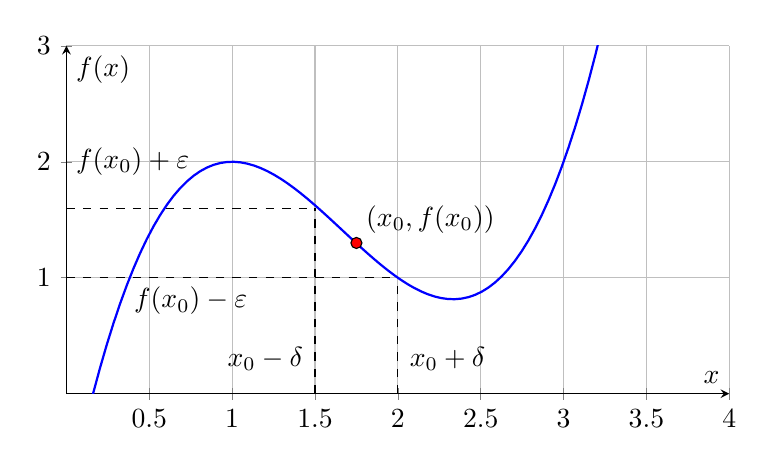
\begin{tikzpicture}
    \begin{axis}[
        axis lines = middle,
        xlabel = \(x\),
        ylabel = {\(f(x)\)},
        domain=0:4,
        samples=100,
        ymin=0, ymax=3,
        xmin=0, xmax=4,
        width=10cm,
        height=6cm,
        grid=both,
    ]
    \addplot[blue, thick] {(x-1)^3 -2*(x-1)^2+ 2};
    \draw[dashed] (1.5,0) -- (1.5,1.6);
    \draw[dashed] (2,0) -- (2,1);
    \draw[dashed] (0,1) -- (2,1);
    \draw[dashed] (0,1.6) -- (1.5,1.6);
    \draw[fill=red] (1.75,1.3) circle (2pt) node[anchor=south west] {\( (x_0, f(x_0)) \)};
    \node at (0.75, 0.8) {\(f(x_0) - \varepsilon\)};
    \node at (0.4, 2) {\(f(x_0) + \varepsilon\)};
    \node at (1.2, 0.3) {\(x_0 - \delta\)};
    \node at (2.3, 0.3) {\(x_0 + \delta\)};
    \end{axis}
\end{tikzpicture}
\end{center}

\subsubsection{Neighborhoods}
A \textit{neighborhood} of a set $A$ is any open set that contains $A$. If $(X, \mathcal{T}_X)$ and $(Y, \mathcal{T}_Y)$ are topological spaces, and $f: X \to Y$ is a mapping, then $f$ is continuous at a point $x_0 \in X$ if for every neighborhood $V$ of $f(x_0)$ in $Y$, there exists a neighborhood $U$ of $x_0$ in $X$ such that:
\[f(U) \subset V.\]

\subsubsection*{Observation}
This is equivalent to the $\varepsilon$-$\delta$ definition on the $\mathbb{R}^n$ spaces.

\subsubsection{Global Continuity}
If $(X, \mathcal{T}_X)$ and $(Y, \mathcal{T}_Y)$ are topological spaces and $f: X \to Y$ is a mapping, then $f$ is globally continuous if:
\[f^{-1}(V) = \{x \in X : f(x) \in V\} \in \mathcal{T}_X, \quad \forall V \in \mathcal{T}_Y.\]
where $f^{-1}(V)$ is the preimage of $V$ under $f$.

\begin{center}
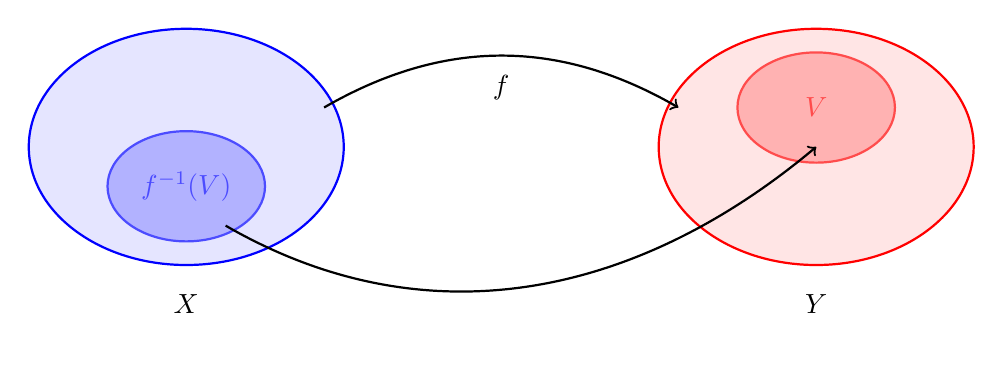
\begin{tikzpicture}
    % Draw blobs for X and Y
    \draw[thick, blue, fill=blue!10] (-2, -1.5) ellipse (2 and 1.5) node {};
    \node at (-2, -3.5) {\(X\)};
    \draw[thick, red, fill=red!10] (6, -1.5) ellipse (2 and 1.5) node {};
    \node at (6, -3.5) {\(Y\)};

    % Sub-blobs for T_X and T_Y
    \draw[thick, blue!70, fill=blue!30] (-2, -2) ellipse (1 and 0.7) node {\(f^{-1}(V)\)};
    \draw[thick, red!70, fill=red!30] (6, -1) ellipse (1 and 0.7) node {\(V\)};

    % Arrows between X and Y
    \draw[->, thick, in=150, out=30] (-0.25, -1) to (4.25, -1);
    \draw[->, thick, in=220, out=330] (-1.5, -2.5) to (6, -1.5);
    \node at (2, -0.75) {\(f\)};
    \node at (2, -3) {\(\)};
\end{tikzpicture}
\end{center}

So, $f$ is continuous if the preimage of every open set in $Y$ is an open set in $X$.

\subsubsection{Proposition}
If $(X, \mathcal{T}_X)$ and $(Y, \mathcal{T}_Y)$ are topological spaces and $f: X \to Y$ is a mapping, then $f$ is continuous if it is continuous at every point $x \in X$.

\subsection{Measurable Spaces}
A collection $\mathcal{A}$ of subsets of a space $X$ is a \textit{$\sigma$-algebra} if:
\begin{enumerate}
    \item $\emptyset \in \mathcal{A}$.
    \item If $A \in \mathcal{A}$, then $A^C\in \mathcal{A}$.
    \item If $\{A_j\}_{j \in \mathbb{N}}$ is a countable collection with each $A_j \in \mathcal{A}$, then:
    \[\bigcup_{j=1}^{\infty} A_j \in \mathcal{A}\]
\end{enumerate}

The sets of $\mathcal{A}$ are called \textit{measurable sets}. The pair $(X, \mathcal{A})$ is called a \textit{measurable space}. If the third property holds for finite collections, then $\mathcal{A}$ is called an \textit{algebra}.

\subsubsection*{Example}
Is $\mathbb{R}$ with the topology of the usual open sets a $\sigma$-algebra?
No, because
\[(a, b) \in \mathcal{T} \text{ but } (a, b)^C = (-\infty, a] \cup [b, \infty) \notin \mathcal{T}.\]

\subsubsection*{Example}
The collection $\mathcal{P}(X)$, the power set of $X$, is a $\sigma$-algebra on $X$.

On $X$, the collection $\{\emptyset, X\}$ is the smallest $\sigma$-algebra.

\subsubsection{Properties of measurable spaces}
If $(X, \mathcal{A})$ is a measurable space, then:
\begin{enumerate}
    \item If $\emptyset \in \mathcal{A}$, then $\emptyset ^C = X \in \mathcal{A}$.
    \item If $A_1, A_2, \ldots, A_n \in \mathcal{A}$, then:
    \[\bigcup_{j=1}^{n} A_j \in \mathcal{A}.\]
    \item If $\{A_j\}_{j \in \mathbb{N}}$ is a countable collection with each $A_j \in \mathcal{A}$ then, following the second property of $\sigma$-algebras:
    \[A_j^C \in \mathcal{A}, \quad \forall j \in \mathbb{N}.\]
    Then, by the third property of $\sigma$-algebras:
    \[\bigcup_{j=1}^{\infty} A_j^C \in \mathcal{A}.\]
    Finally, by the second property again:
    \[\left(\bigcup_{j=1}^{\infty} A_j^C\right)^C = \bigcap_{j=1}^{\infty} A_j \in \mathcal{A}.\]
    \item If $A, B \in \mathcal{A}$, then:
    \[A \setminus B = A \cap B^C \in \mathcal{A}.\]
\end{enumerate}

\subsubsection{Proposition}
If $S \subset \mathcal{P}(X)$, then $\sigma(S)$ is called the $\sigma$-algebra generated by $S$:
\[\sigma(S) = \mathcal{A}_S = \bigcap \{\mathcal{A} : \mathcal{A} \text{ is a } \sigma\text{-algebra and } S \subseteq \mathcal{A} \subseteq \mathcal{P}(X)\}.\]

\subsubsection*{Example}
Let $X = \{1, 2, 3, 4\}$ and $S = \{\{1\}, \{3, 4\}\}$. Then:
\[\sigma(S) = \{\emptyset, X, \{1\}, \{2, 3, 4\}, \{3, 4\}, \{1, 2\}, \{2\}, \{1, 3, 4\}\}.\]

\subsubsection{Borel $\sigma$-algebra}
The Borel $\sigma$-algebra on $X$, denoted by $\mathcal{B}(X)$, is the $\sigma$-algebra generated by the open sets of $X$, 
\[\mathcal{B}(X) = \sigma(\mathcal{T}(X)).\]
Its elements are called \textit{Borel sets}.

\subsubsection*{Example}
The Borel $\sigma$-algebra on $\mathbb{R}$, $\mathcal{B}(\mathbb{R})$, contains all open intervals, closed intervals, countable sets, and complements of these sets. Examples of these Borel sets include:
\[(a, b), \quad [a, b], \quad (a, b], \quad [a, b), \quad \mathbb{Q}, \quad \mathbb{R} \setminus \mathbb{Q}, \quad \{x\}, \quad \mathbb{R}, \quad \emptyset.\]

\section{Measurable functions and Integration}
A mapping $f: (X, \mathcal{A}) \to (Y, \mathcal{T})$, where $(X, \mathcal{A})$ is a measurable space and $(Y, \mathcal{T})$ is a topological space, is said to be a \textit{measurable function} if the preimage of every open set in $Y$ is a measurable set in $X$. Formally, for every open set $V \in \mathcal{T}_Y$, we have:
\[f^{-1}(V) = \{x \in X : f(x) \in V\} \in \mathcal{A}.\]

\subsubsection*{Observation}
A mapping $f: (X, \mathcal{T}_X) \to (Y, \mathcal{T}_Y)$ between two topological spaces is continuous if 
\[ \forall V \in \mathcal{T}_Y, \quad f^{-1}(V) \in \mathcal{T}_X.\]

\subsubsection*{Example}
If \( (X, \mathcal{A}) \) is a measurable space and \( A \in \mathcal{A} \), then the characteristic function \( \chi_A: X \to \{0, 1\} \) defined by:
\[\chi_A(x) = \begin{cases} 1 & \text{if } x \in A, \\ 0 & \text{if } x \notin A, \end{cases}\]
is a measurable function.
\vskip 1em
Now, let us consider $f : (X, \mathcal{A}) \to (\mathbb{R}, \mathcal{T})$. For any $V \in \mathcal{T}$, we have:
\[V = (a, b) \quad \text{or} \quad V = (a, b) \cup (c, d) \cup \ldots\]
Then, we can analyze the preimage of $V$ under $f$:
\[f^{-1}(V) = \begin{cases}
    A, & \text{if } 1 \in V \\
    X \setminus A, & \text{if } 1 \notin V \\
\end{cases}\]
Since both $A$ and $X \setminus A$ are in $\mathcal{A}$, it follows that $\chi_A$ is a measurable function.

\subsubsection*{Example}
Let $X = \{1, 2, 3\}$ and $\mathcal{A} = \{\emptyset, X \}$. Define $f: X \to \mathbb{R}$ by:
\[f(1) = f(2) = f(3) = 5.\]
Then, for any open set $V \subset \mathbb{R}$:
\[f^{-1}(V) = \begin{cases}
    X, & \text{if } 5 \in V \\
    \emptyset, & \text{if } 5 \notin V \\
\end{cases}\]
Since both $X$ and $\emptyset$ are in $\mathcal{A}$, $f$ is a measurable function.

\begin{center}
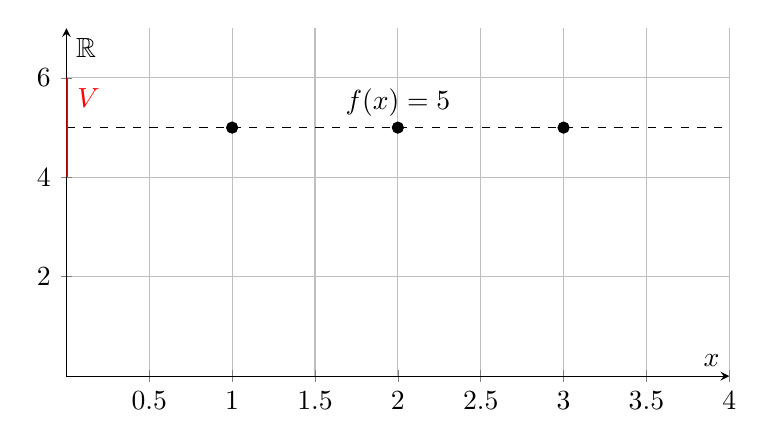
\begin{tikzpicture}
    \begin{axis}[
        axis lines = middle,
        xlabel = \(x\),
        ylabel = {\(\mathbb{R}\)},
        ymin=0, ymax=7,
        xmin=0, xmax=4,
        width=10cm,
        height=6cm,
        grid=both,
    ]
    \addplot[only marks, mark=*, mark size=2pt] coordinates {
        (1,5) (2,5) (3,5)
    };
    \draw[dashed] (0,5) -- (4,5);
    \node at (2, 5.5) {\(f(x) = 5\)};
    \draw[red, very thick] (0,4) -- (0,6) node[anchor=north west] {\(V\)};
    \end{axis}
\end{tikzpicture}
\end{center}

\subsection{Composition of Functions and Measurability}
Consider two topological spaces \((Y, \mathcal{T}_Y)\) and \((Z, \mathcal{T}_Z)\), and a \textit{continuous} function \(g: Y \to Z\):
\begin{enumerate}
    \item If $(X, \mathcal{T}_X)$ is a \textit{topological space} and $f: X \to Y$ is \textit{continuous}, then the composition \(h = g \circ f: X \to Z\) is continuous.
    \item If $(X, \mathcal{A})$ is a \textit{measurable space} and $f: X \to Y$ is \textit{measurable}, then the composition \(h = g \circ f: X \to Z\) is measurable.
    \end{enumerate}
\begin{center}
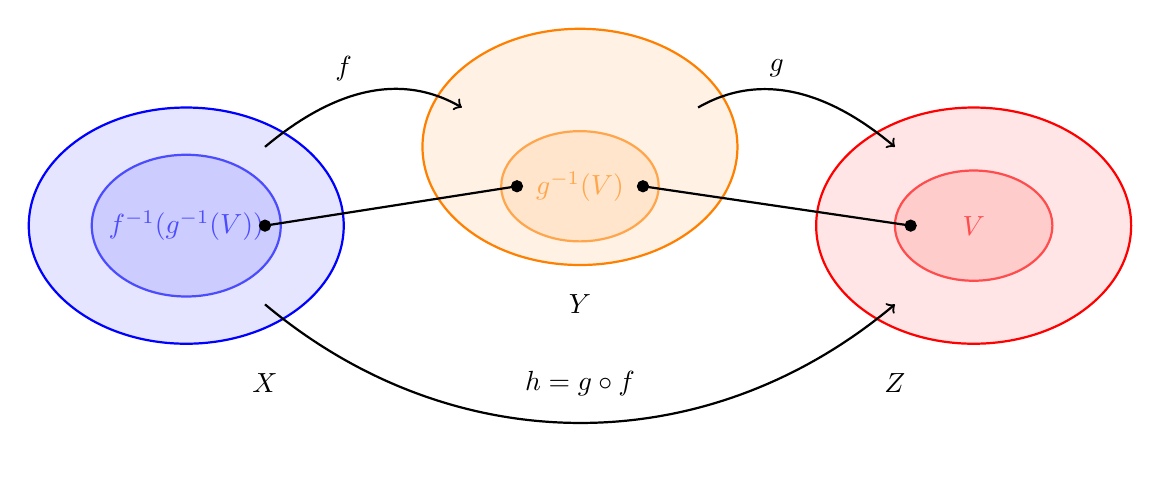
\begin{tikzpicture}
    % Draw blobs for X, Y, and Z
        \draw[thick, blue, fill=blue!10] (-3, -2.5) ellipse (2 and 1.5) node {};
        \node at (-2, -4.5) {\(X\)};
        \draw[thick, orange, fill=orange!10] (2, -1.5) ellipse (2 and 1.5) node {};
        \node at (2, -3.5) {\(Y\)};
        \draw[thick, red, fill=red!10] (7, -2.5) ellipse (2 and 1.5) node {};
        \node at (6, -4.5) {\(Z\)};
        % Sub-blobs for T_X, T_Y, and T_Z
        \draw[thick, orange!70, fill=orange!20] (2, -2) ellipse (1 and 0.7) node {\(g^{-1}(V)\)};
        \draw[thick, blue!70, fill=blue!20] (-3, -2.5) ellipse (1.2 and 0.9) node {\(f^{-1}(g^{-1}(V))\)};
        \draw[thick, red!70, fill=red!20] (7, -2.5) ellipse (1 and 0.7) node {\(V\)};
        % Arrows between X, Y, and Z
        \draw[->, thick, in=150, out=40] (-2, -1.5) to (0.5, -1);
        \draw[->, thick, in=140, out=30] (3.5, -1) to (6, -1.5);
        \draw[->, thick, in=220, out=320] (-2, -3.5) to (6, -3.5);
        \node at (-1, -0.5) {\(f\)};
        \node at (4.5, -0.5) {\(g\)};
        \node at (2, -4.5) {\(h = g \circ f\)};
        \draw[.-., thick] (-2, -2.5) to (1.2, -2);
        \draw[fill=black] (-2, -2.5) circle (2pt); % Point at the end
        \draw[fill=black] (1.2, -2) circle (2pt); % Point at the end
        \draw[.-., thick] (2.8, -2) to (6.2, -2.5);
        \draw[fill=black] (2.8, -2) circle (2pt); % Point at the end
        \draw[fill=black] (6.2, -2.5) circle (2pt); % Point at the end
\end{tikzpicture}
\end{center}

\begin{proof}
Consider any open set \(V \in \mathcal{T}_Z\). Since \(g\) is continuous, the preimage \(g^{-1}(V) \in \mathcal{T}_Y\) (it is also an open set, now in \(\mathcal{T}_Y\)). And then, \(f^{-1}(g^{-1}(V)) \in \mathcal{T}_X\) (that is, it is an open set in \(\mathcal{T}_X\)).
    Observe that the preimage of \(g^{-1}(V)\) under \(f\) is:
    \[h^{-1}(V) = (g \circ f)^{-1}(V) = f^{-1}(g^{-1}(V)).\]

    Now consider any open set \(V \in \mathcal{T}_Z\). Since \(g\) is continuous, the preimage \(g^{-1}(V) \in \mathcal{T}_Y\). And then, \(f^{-1}(g^{-1}(V)) \in \mathcal{A}\) (that is, it is a measurable set in \(\mathcal{A}\)).
\end{proof}

\subsubsection*{Example}
On \(\mathbb{R}\) with \(\mathcal{T}\) the topology of the open sets, the Borel \(\sigma\)-algebra \(\mathcal{B}(\mathbb{R})\) is generated by the open sets of \(\mathbb{R}\). Then \((\mathbb{R}, \mathcal{B}(\mathbb{R}))\) is a measurable space.

\subsection{Theorem: Characterizations of Measurable Functions}
Given a measurable space \((X, \mathcal{A})\) and \(f : X \to \mathbb{R}\), the following statements are equivalent:
\begin{enumerate}
    \item \(f\) is measurable.
    \item For every \(a \in \mathbb{R}\), the set \(\{x \in X : f(x) > a\} \in \mathcal{A}\).
    \item For every \(a \in \mathbb{R}\), the set \(\{x \in X : f(x) \geq a\} \in \mathcal{A}\).
    \item For every \(a \in \mathbb{R}\), the set \(\{x \in X : f(x) < a\} \in \mathcal{A}\).
    \item For every \(a \in \mathbb{R}\), the set \(\{x \in X : f(x) \leq a\} \in \mathcal{A}\).
    \item For every \(a, b \in \mathbb{R}\) with \(a < b\), the set \(\{x \in X : a < f(x) < b\} \in \mathcal{A}\).
    \item The preimage of every open, closed, or Borel set in \(\mathbb{R}\) is in \(\mathcal{A}\).
\end{enumerate}

\subsection{Lemma}
Given a measurable function \(f : (X, \mathcal{A}) \to (\mathbb{R}, \mathcal{T})\), the family of sets:
\[\mathcal{A}_f = \{B \in \mathbb{R} : f^{-1}(B) \in \mathcal{A}\}\]
is a \(\sigma\)-algebra on \(\mathbb{R}\), and it is called the \textit{image \(\sigma\)-algebra}. Then \(\mathcal{A}_f\) contains the Borel \(\sigma\)-algebra \(\mathcal{B}(\mathbb{R})\) because by definition, 
\[(a, \infty) \in \mathcal{A}_f \quad \text{for all } a \in \mathbb{R}.\]

\begin{proof}
To show that \(\mathcal{A}_f\) is a \(\sigma\)-algebra, we need to verify the three properties:
\begin{enumerate}
    \item Since \(f^{-1}(\emptyset) = \emptyset\) and \(\emptyset \in \mathcal{A}\), we have \(\emptyset \in \mathcal{A}_f\).
    \item If \(B \in \mathcal{A}_f\), then \(f^{-1}(B) \in \mathcal{A}\). Since \(\mathcal{A}\) is a \(\sigma\)-algebra, \(f^{-1}(B)^C = f^{-1}(B^C) \in \mathcal{A}\). Thus, \(B^C \in \mathcal{A}_f\).
    \item If \(\{B_j\}_{j \in \mathbb{N}}\) is a countable collection with each \(B_j \in \mathcal{A}_f\), then \(f^{-1}(B_j) \in \mathcal{A}\) for all \(j\). Since \(\mathcal{A}\) is a \(\sigma\)-algebra, we have:
    \[\bigcup_{j=1}^{\infty} f^{-1}(B_j) = f^{-1}\left(\bigcup_{j=1}^{\infty} B_j\right) \in \mathcal{A}.\]
    Therefore, \(\bigcup_{j=1}^{\infty} B_j \in \mathcal{A}_f\).
\end{enumerate}
\end{proof}

\subsection{Measure and Measure Space}
A \textit{measure} on a measurable space \((X, \mathcal{A})\) is a function \(\mu: \mathcal{A} \to [0, \infty]\) such that:
\begin{enumerate}
    \item \(\mu(\emptyset) = 0\).
    \item If \(\{A_j\}_{j \in \mathbb{N}}\) is a countable collection of pairwise disjoint sets in \(\mathcal{A}\), then:
    \[\mu\left(\bigcup_{j=1}^{\infty} A_j\right) = \sum_{j=1}^{\infty} \mu(A_j).\]
\end{enumerate}

The triple \((X, \mathcal{A}, \mu)\) is called a \textit{measure space}.

\subsubsection*{Observation}
Also, there exist negative measures, where \(\mu: \mathcal{A} \to [-\infty, \infty]\), and complex measures, where \(\mu: \mathcal{A} \to \mathbb{C}\). Furthermore, if \(\mu(X) = 1\), then \((X, \mathcal{A}, \mu)\) is called a \textit{probability space}.

\subsubsection*{Example}
Consider the space \(X = \{1, 2, 3\}\) and the \(\sigma\)-algebra \(\mathcal{A} = \{\emptyset, X, \{1, 2\}, \{3\}\}\). Define the measure \(\mu: \mathcal{A} \to [0, \infty)\) by:
\[\mu(\emptyset) = \mu(\{1, 2\}) = 0, \quad \mu(X) = \mu(\{3\}) = 1.\]
Observe that \((X, \mathcal{A}, \mu)\) is a probability space. Also, the measure is countably additive since:
\[\mu(X) = 1 = \mu(\{1, 2\}) + \mu(\{3\}) = 0 + 1 = 1.\]

\subsubsection*{Observation}
On any set \(X\) with the \(\sigma\)-algebra \(\mathcal{A}\), we can define a measure \(\mu: \mathcal{A} \to [0, \infty]\) using a weight function:
\[p : X \to [0, \infty], \quad p(x) \text{ is the weight of } x.\]
If \(A \in \mathcal{A}\), then:
\[\mu(A) = \sum_{x \in A} p(x) := \sup_{\{x_1, \ldots, x_n\} \subseteq A} \sum_{j=1}^{n} p(x_j).\]

\subsubsection*{Example}
On \((\mathbb{N}, \mathcal{P}(\mathbb{N}))\), we can use the weight function \(p(x) = 1, \forall x \in \mathbb{N}\). Then, we obtain the \textit{counting measure}:
\[\mu(A) = \sum_{x \in A} 1 = \card{A}.\]

\subsubsection*{Example}
Now let \(p(x) = 1\) for \(x = a\), and \(p(x) = 0\) for \(x \neq a\). Then, we obtain the \textit{Dirac-\(\delta\) measure} at \(a\):
\[\mu(A) = \sum_{x \in A} p(x) = \begin{cases} 1 & \text{if } a \in A, \\ 0 & \text{if } a \notin A. \end{cases}\]

\subsection{Theorem: Properties of Measures}
Let \((X, \mathcal{A}, \mu)\) be a measure space. Then, 
\begin{enumerate}
    \item If \(A_1, A_2, \ldots, A_n \in \mathcal{A}\) disjoint, then:
    \[\mu\left(\bigcup_{j=1}^{n} A_j\right) = \sum_{j=1}^{n} \mu(A_j).\]
    \begin{proof}
        Define \(\emptyset = A_{n+1}, A_{n+2}, \ldots\). Then, by the properties of measures:
        \[\mu\left(\bigcup_{j=1}^{\infty} A_j\right) = \sum_{j=1}^{\infty} \mu(A_j) = \sum_{j=1}^{n} \mu(A_j) + \sum_{j=n+1}^{\infty} \mu(\emptyset) = \sum_{j=1}^{n} \mu(A_j) + 0 = \sum_{j=1}^{n} \mu(A_j).\]
    \end{proof}
    \item If \(A, B \in \mathcal{A}\) and \(A \subseteq B\), then:
    \[\mu(A) \leq \mu(B).\]
    And if \(\mu(A) < \infty\), then:
    \[\mu(B \setminus A) = \mu(B) - \mu(A).\]
    \begin{proof}
        Since \(A \subseteq B\), we can write \(B = A \cup (B \setminus A)\) with \(A\) and \(B \setminus A\) disjoint. Then, by the properties of measures:
        \[\mu(B) = \mu(A) + \mu(B \setminus A) \geq \mu(A).\]
        If \(\mu(A) < \infty\), then rearranging gives:
        \[\mu(B \setminus A) = \mu(B) - \mu(A).\]
    \end{proof}
    \item If \(\{A_j\}_{j \in \mathbb{N}}\) is a sequence of sets in \(\mathcal{A}\) (i.e., \(A_1 \subseteq A_2 \subseteq A_3 \subseteq \ldots\)), then:
    \[\mu\left(\bigcup_{j=1}^{\infty} A_j\right) \leq \sum_{j=1}^{\infty} \mu(A_j).\]
    \item If \(\{A_j\}_{j \in \mathbb{N}}\) is a sequence of increasing sets in \(\mathcal{A}\) (i.e., \(A_1 \subseteq A_2 \subseteq A_3 \subseteq \ldots\)), then:
    \[\mu\left(\bigcup_{j=1}^{\infty} A_j\right) = \lim_{n \to \infty} \mu(A_n) = \sup_{n \in \mathbb{N}} \mu(A_n).\]
    \item If \(\{A_j\}_{j \in \mathbb{N}}\) is a sequence of decreasing sets in \(\mathcal{A}\) (i.e., \(A_1 \supseteq A_2 \supseteq A_3 \supseteq \ldots\)) and \(\mu(A_1) < \infty\), then:
    \[\mu\left(\bigcap_{j=1}^{\infty} A_j\right) = \lim_{n \to \infty} \mu(A_n) = \inf_{n \in \mathbb{N}} \mu(A_n).\]
    
\end{enumerate}

\subsubsection*{Example}
Let \(X = \mathbb{N}\) and \(A_n = \{n, n+1, n+2, \ldots\}\). Consider the counting measure \(\mu\) on \(\mathcal{A} = \mathcal{P}(\mathbb{N})\). Then:
\[A_1 \supset A_2 \supset A_3 \supset \ldots \quad \text{and} \quad \bigcap_{n=1}^{\infty} A_n = \emptyset.\]
Thus:
\[\mu\left(\bigcap_{n=1}^{\infty} A_n\right) = \mu(\emptyset) = 0.\]
However, \(\mu(A_1) = \infty\), so the condition \(\mu(A_1) < \infty\) is necessary.

\subsection{Completion of Measure Spaces}
A property is said to hold \textit{almost everywhere} (a.e.) if it holds everywhere except on a set of measure zero. A set with measure zero is called a \textit{null set}. 

\subsubsection*{Example}
Consider the space \(X = \{1, 2, 3\}\) with the \(\sigma\)-algebra \(\mathcal{A} = \{\emptyset, X, \{1, 2\}, \{3\}\}\) and the measure \(\mu: \mathcal{A} \to [0, \infty)\) defined by:
\[\mu(\emptyset) = \mu(\{1, 2\}) = 0, \quad \mu(X) = \mu(\{3\}) = 1.\]
Then, the set \(\{1, 2\}\) is a null set since \(\mu(\{1, 2\}) = 0\), and \((X, \mathcal{A}, \mu)\) is a measure space.

Let us define the functions \(f, g: X \to \mathbb{R}\) by:
\[f(1) = f(2) = f(3) = 3, \quad g(x) = x.\]
Then, \(f(x) = g(x)\) almost everywhere since they differ only on the null set \(\{1, 2\}\).
However, \(f\) is measurable while \(g\) is not, because:
\[g^{-1}((2, 4)) = \{3\} \in \mathcal{A},\]
but
\[g^{-1}((0, 2)) = \{1\} \notin \mathcal{A}.\]

A measure space \((X, \mathcal{A}, \mu)\) is said to be \textit{complete} if every subset \(E\) of a null set \(N\) is measurable. 
\[\forall N \in \mathcal{A} \text{ with } \mu(N) = 0, \quad \forall E \subseteq N, \quad E \in \mathcal{A}.\]

\subsubsection*{Example}
Consider \(X = \mathbb{N}\) with the \(\sigma\)-algebra \(\mathcal{A} = \mathcal{P}(\mathbb{N})\) and a counting measure \(\mu\). Since the only null set is \(\emptyset\), every subset of a null set is measurable. Thus, \((\mathbb{N}, \mathcal{P}(\mathbb{N}), \mu)\) is a complete measure space.
\vskip 1em
Now, consider a Dirac-\(\delta\) measure \(\mu\) at \(a \in \mathbb{R}\) on \(\mathcal{P}(\mathbb{R})\). The Dirac measure is defined by:
\[
\mu(E) = \begin{cases}
1 & \text{if } a \in E, \\
0 & \text{if } a \notin E.
\end{cases}
\]
In this case, the null set is \(\emptyset\), and every subset of \(\emptyset\) is measurable. Thus, \((\mathbb{R}, \mathcal{P}(\mathbb{R}), \mu)\) is also a complete measure space.


\subsection{Theorem: Completion of a Measure Space}
Given a measure space \((X, \mathcal{A}, \mu)\), we can construct its completion \((X, \overline{\mathcal{A}}, \overline{\mu})\) as follows:
\begin{enumerate}
    \item Define \(\mathcal{N} = \{N \in \mathcal{A} : \mu(N) = 0\}\) as the collection of null sets.
    \item Define \(\overline{\mathcal{A}} = \{A \cup N : A \in \mathcal{A}, N \in \mathcal{N}\}\) as the collection of sets formed by the union of a measurable set and a null set.
    \item Define \(\overline{\mu}: \overline{\mathcal{A}} \to [0, \infty]\) by:
    \[\overline{\mu}(A \cup N) = \mu(A), \quad \text{for } A \in \mathcal{A}, N \in \mathcal{N}.\]
\end{enumerate}
Then, \((X, \overline{\mathcal{A}}, \overline{\mu})\) is a complete measure space.
Furthermore, \(\overline{\mathcal{A}}\) is the smallest \(\sigma\)-algebra containing \(\mathcal{A}\), and \(\overline{\mu}\) is a complete measure extending \(\mu\).

\begin{proof}
To show that \(\overline{\mathcal{A}}\) is a \(\sigma\)-algebra, we need to verify the three properties:
\begin{enumerate}
    \item Since \(\emptyset \in \mathcal{A}\) and \(\emptyset \in \mathcal{N}\), we have \(\emptyset = \emptyset \cup \emptyset \in \overline{\mathcal{A}}\).
    \item If \(B = A \cup N \in \overline{\mathcal{A}}\) with \(A \in \mathcal{A}\) and \(N \in \mathcal{N}\), then:
    \[B^C = (A \cup N)^C = A^C \cap N^C = (A^C \cap X) \cup (A^C \cap N^C).\]
    Since \(A^C \in \mathcal{A}\) and \(N^C \in \mathcal{A}\), we have \(B^C \in \overline{\mathcal{A}}\).
    \item If \(\{B_j\}_{j \in \mathbb{N}}\) is a countable collection with each \(B_j = A_j \cup N_j \in \overline{\mathcal{A}}\), where \(A_j \in \mathcal{A}\) and \(N_j \in \mathcal{N}\), then:
    \[
    \bigcup_{j=1}^{\infty} B_j = \bigcup_{j=1}^{\infty} (A_j \cup N_j) = \left(\bigcup_{j=1}^{\infty} A_j\right) \cup \left(\bigcup_{j=1}^{\infty} N_j\right).
    \]
    Since \(\bigcup_{j=1}^{\infty} A_j \in \mathcal{A}\) and \(\bigcup_{j=1}^{\infty} N_j \in \mathcal{N}\), we have \(\bigcup_{j=1}^{\infty} B_j \in \overline{\mathcal{A}}\). 
\end{enumerate}
Now we need to check wether \(\overline{\mu}\) is well-defined on \(\overline{\mathcal{A}}\) and satisfies the properties of a measure:
\begin{enumerate}
    \item For any \(B = A \cup N \in \overline{\mathcal{A}}\) with \(A \in \mathcal{A}\) and \(N \in \mathcal{N}\), we have:
    \[\overline{\mu}(B) = \overline{\mu}(A \cup N) = \mu(A) \geq 0.\]
    \item If \(\{B_j\}_{j \in \mathbb{N}}\) is a countable collection of pairwise disjoint sets in \(\overline{\mathcal{A}}\), where \(B_j = A_j \cup N_j\) with \(A_j \in \mathcal{A}\) and \(N_j \in \mathcal{N}\), then:
    \[\bigcup_{j=1}^{\infty} B_j = \left(\bigcup_{j=1}^{\infty} A_j\right) \cup \left(\bigcup_{j=1}^{\infty} N_j\right).\]
    Since the \(B_j\) are pairwise disjoint, the \(A_j\) are also pairwise disjoint. Thus, by the properties of measures:
    \[\overline{\mu}\left(\bigcup_{j=1}^{\infty} B_j\right) = \mu\left(\bigcup_{j=1}^{\infty} A_j\right) = \sum_{j=1}^{\infty} \mu(A_j) = \sum_{j=1}^{\infty} \overline{\mu}(B_j).\]
\end{enumerate}
\end{proof}

\subsubsection*{Example}
Consider the space \(X = \{1, 2, 3\}\) with the \(\sigma\)-algebra \(\mathcal{A} = \{\emptyset, X, \{1, 2\}, \{3\}\}\) and the measure \(\mu: \mathcal{A} \to [0, \infty)\) defined by:
\[\mu(\emptyset) = \mu(\{1, 2\}) = 0, \quad \mu(X) = \mu(\{3\}) = 1.\]
Then, the null set is \(\mathcal{N} = \{\emptyset, \{1, 2\}\}\). The completion of the measure space is given by:
\[\overline{\mathcal{A}} = \{A \cup N : A \in \mathcal{A}, N \in \mathcal{N}\} = \{\emptyset, \{1\}, \{2\}, \{1, 2\}, \{3\}, \{1, 3\}, \{2, 3\}, X\} = \mathcal{P}(X).\]
The completed measure \(\overline{\mu}: \overline{\mathcal{A}} \to [0, \infty)\) is defined by:
\[\overline{\mu}(\emptyset) = \overline{\mu}(\{1\}) = \overline{\mu}(\{2\}) = \overline{\mu}(\{1, 2\}) = 0, \quad \overline{\mu}(\{3\}) = \overline{\mu}(\{1, 3\}) = \overline{\mu}(\{2, 3\}) = \overline{\mu}(X) = 1.\]

\subsection{Semi-algebra}
A collection \(\mathcal{E} \subseteq \mathcal{P}(X)\) is called a \textit{semi-algebra} if:
\begin{enumerate}
    \item \(\emptyset \in \mathcal{E}\).
    \item If \(A, B \in \mathcal{E}\), then \(A \cap B \in \mathcal{E}\).
    \item If \(A \in \mathcal{E}\), then \(A^C = B_1 \cup B_2 \cup \ldots \cup B_n\) where \(B_j \in \mathcal{E}\) for \(j = 1, 2, \ldots, n\).
\end{enumerate}

\subsubsection*{Example}
On \(\mathbb{R}\), the collection of all intervals of the form:
\[(a, b), \quad [a, b), \quad (a, b], \quad [a, b], \quad (-\infty, a), \quad (-\infty, a], \quad (a, \infty), \quad [a, \infty),\]
where \(a, b \in \mathbb{R}\), is a semi-algebra.
\vskip 1em
A set function \(\mu: X \to [0, \infty]\) is \textit{\(\sigma\)-finite} if 
\[X = \bigcup_{j=1}^{\infty} X_j, \quad X_j \in X, \quad \mu(X_j) < \infty \text{ for all } j.\]
and we say that \(X\) is \(\sigma\)-finite with respect to \(\mu\).

\subsection{Operations with infinity}
The following conventions are used when dealing with infinity in measure theory:
\begin{itemize}
    \item \(a + \infty = \infty + a = \infty\) for any \(a \in [0, \infty]\).
    \item \(a \cdot \infty = \infty \cdot a = \infty\) for any \(a \in (0, \infty]\).
    \item \(0 \cdot \infty = \infty \cdot 0 = 0\).
    \item Cancellation law: If \(a, b \in [0, \infty]\) and \(c \in (0, \infty]\), then:
    \[a + c = b + c \implies a = b.\]
    \item If \(a, b \in [0, \infty]\) and \(c \in (0, \infty)\), then:
    \[a \cdot c = b \cdot c \implies a = b.\]
\end{itemize}

\subsection{Outer Measure}
An \textit{outer measure} on a set \(X\) is a function \(\mu^*: \mathcal{P}(X) \to [0, \infty]\) such that:
\begin{enumerate}
    \item \(\mu^*(\emptyset) = 0\).
    \item If \(A \subseteq B \subseteq X\), then \(\mu^*(A) \leq \mu^*(B)\).
    \item If \(\{A_j\}_{j \in \mathbb{N}} \subseteq \mathcal{P}(X)\), then:
    \[\mu^*\left(\bigcup_{j=1}^{\infty} A_j\right) \leq \sum_{j=1}^{\infty} \mu^*(A_j).\]
\end{enumerate}

\subsubsection*{Example}
Consider the set \(X = \{1, 2, 3\}\) and define the function \(\mu^*: \mathcal{P}(X) \to [0, \infty]\) by:
\[\mu^*(A) = \begin{cases} 0 & \text{if } A = \emptyset, \\ 1 & \text{if } A \neq \emptyset. \end{cases}\]
Then, \(\mu^*\) is an outer measure on \(X\) since it satisfies the three properties:
\begin{enumerate}
    \item \(\mu^*(\emptyset) = 0\).
    \item If \(A \subseteq B\), then:
    \[\mu^*(A) \leq \mu^*(B)\] holds trivially since both sides are either 0 or 1.
    \item For any collection \(\{A_j\}_{j \in \mathbb{N}}\), we have:
    \[\mu^*\left(\bigcup_{j=1}^{\infty} A_j\right) \leq \sum_{j=1}^{\infty} \mu^*(A_j)\] since the left side is either 0 or 1, and the right side is at least 0.
\end{enumerate}

\subsubsection*{Remark}
Given an outer measure \(\mu^*\) on a set \(X\), a set \(A \subseteq X\) is said to be \textit{\(\mu^*\)-measurable} if:
\[\mu^*(E) = \mu^*(E \cap A) + \mu^*(E \cap A^C) \quad \text{for all } E \subseteq X.\]

\subsection{Caratheodory-Hopf's Theorem}
Consider \(\mathcal{M} = \{M \subseteq X : M \text{ is } \mu^*\text{-measurable}\}\). Then:
\begin{enumerate}
    \item \(\mathcal{M}\) is a \(\sigma\)-algebra.
    \item The restriction \(\mu = \mu^*|_{\mathcal{M}}\) is a complete measure on \(\mathcal{M}\).
\end{enumerate}

To define an outer measure, we can start with a semi-algebra. Consider a semi-algebra \(\mathcal{E} \subseteq \mathcal{P}(X)\) and a countably additive function \(\mu_0: \mathcal{E} \to [0, \infty]\). Then, we can define an outer measure \(\mu^*\) for all \(A \subseteq \mathcal{P}(X)\):
\[\mu^*(A) = \inf\left\{\sum_{j=1}^{\infty} \mu_0(E_j) : A \subseteq \bigcup_{j=1}^{\infty} E_j, E_j \in \mathcal{E}\right\}.\]

and define \(\mathcal{M} = \{M \subseteq X : M \text{ is } \mu^*\text{-measurable}\}\). Then:
\begin{enumerate}
    \item \(\mu^*\) is an outer measure and \(\mu^*|_{\mathcal{M}} = \mu\) is a complete measure on \(\mathcal{M}\), where \(\mu\) extends \(\mu_0\).
    \item If \(\mu_0\) is \(\sigma\)-finite, then \(\mu\) is the unique extension of \(\mu_0\) to a measure on \(\sigma(\mathcal{E})\).
\end{enumerate}

\begin{center}
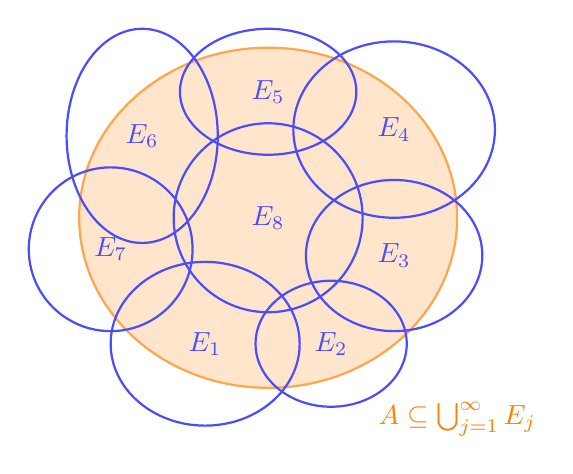
\begin{tikzpicture}[scale=0.8]
        % Draw the set A
        \draw[thick, orange!70, fill=orange!20] (0, 0) ellipse (3 and 2.7) node {};
        % Draw the sets E1, E2, E3, ...
        \draw[thick, blue!70] (-1, -2) ellipse (1.5 and 1.3) node {\(E_1\)};
        \draw[thick, blue!70] (1, -2) ellipse (1.2 and 1) node {\(E_2\)};
        \draw[thick, blue!70] (2, -0.6) ellipse (1.4 and 1.2) node {\(E_3\)};
        \draw[thick, blue!70] (2, 1.4) ellipse (1.6 and 1.4) node {\(E_4\)};
        % Draw the ellipses for E5, E6, ...
        \draw[thick, blue!70] (0, 2) ellipse (1.4 and 1) node {\(E_5\)};
        \draw[thick, blue!70] (-2, 1.3) ellipse (1.2 and 1.7) node {\(E_6\)};
        % Draw the ellipses for E7, E8, ...
        \draw[thick, blue!70] (-2.5, -0.5) ellipse (1.3 and 1.3) node {\(E_7\)};
        \draw[thick, blue!70] (0, 0) ellipse (1.5 and 1.5) node {\(E_8\)};

        % Label the set A
        \node[orange] at (3, -3.2) {\(A \subseteq \bigcup_{j=1}^{\infty} E_j\)};
    \end{tikzpicture}
\end{center}

\subsection{Semi-open Intervals and Elementary Measure}
A \textit{semi-open interval} in \(\mathbb{R}^n\) is a set of the form:
\[I = I_1 \times I_2 \times \ldots \times I_n,\]
where each \(I_j\) is a semi-open interval in \(\mathbb{R}\).
The collection \(\mathcal{E}\) of all semi-open intervals in \(\mathbb{R}^n\) forms a semi-algebra. Furthermore, \(\sigma(\mathcal{E})\) is the Borel \(\sigma\)-algebra \(\mathcal{B}(\mathbb{R}^n)\).
\vskip 1em
The \textit{elementary measure} \(\mu_0\) of a semi-open interval \(I = I_1 \times I_2 \times \ldots \times I_n\) is defined as:
\[\mu_0(I) = \prod_{j=1}^{n} (b_j - a_j),\]
where \(I_j = [a_j, b_j)\) for \(j = 1, 2, \ldots, n\). If any \(I_j\) is of the form \((-\infty, b_j)\) or \([a_j, \infty)\) (i.e., unbounded), we set \(\mu_0(I) = \infty\). Also, \(\mu_0(I_j = \emptyset) = 0\).
This elementary measure \(\mu_0\) is countably additive on the semi-algebra \(\mathcal{E}\). It is \(\sigma\)-finite since:
\[X = \bigcup_{j=1}^{\infty} X_n \quad \text{such that} \quad \mu_0(X_n) < \infty.\]

\subsection{Theorem: Lebesgue Measure}
There exists a unique measure space \((\mathbb{R}^n, \mathcal{M}, m)\) such that
\[\mathcal{M} = \overline{\mathcal{B}(\mathbb{R}^n)} \quad \text{and} \quad m|_{\mathcal{E}} = \mu_0.\]
In particular, 
\begin{enumerate}
    \item \(\forall M \in \mathcal{M}, M = B \cup N\) where \(B \in \mathcal{B}(\mathbb{R}^n)\) and \(N\) is a null set, i.e., \(m(N) = 0\).
    \item \(\forall N \in \mathcal{M}\) with \(m(N) = 0\), there exists \(B \in \mathcal{B}(\mathbb{R}^n)\) such that \(N \subseteq B\) and \(m(B) = 0\).
\end{enumerate}

This unique measure \(m\) is called the \textit{Lebesgue measure} on \(\mathbb{R}^n\). The Lebesgue measure fulfills the following properties:
\begin{enumerate}
    \item Define \(\mathcal{N} = \{N \in \mathcal{M} : m(N) = 0\}\) as the collection of null sets. Then, if \(\{N_k\}_{k=1}^{\infty} \subseteq \mathcal{N}\) is a sequence of null sets, we have:
        \[\bigcup_{k=1}^{\infty} N_k \in \mathcal{N}.\]
    \item If \(a \in \mathbb{R}^n\) is a point, then \(\{a\} \in \mathcal{N}\) and \(m(\{a\}) = 0\).
    \item If \(A \subseteq \mathbb{R}^n\) is countable, then \(A \in \mathcal{N}\) and \(m(A) = 0\).
    \item There exist non-countable sets in \(\mathcal{N}\). For example, the Cantor ternary set \(\mathcal{C} \subseteq [0, 1]\) is uncountable and \(m(\mathcal{C}) = 0\).
    \item If \(H \subseteq \mathbb{R}^n\) is a shifted \((n-1)\)-dimensional hyperplane, then \(H \in \mathcal{N}\) and \(m(H) = 0\).
    \item The Borelian \(\sigma\)-algebra \(\mathcal{B}(\mathbb{R}^n)\) is strictly contained in \(\mathcal{M}\), i.e., \(\mathcal{B}(\mathbb{R}^n) \subsetneq \mathcal{M} \subsetneq \mathcal{P}(\mathbb{R}^n)\).
    \item If \(A \subset \mathbb{R}^n\) is an open set, then \(A \in \mathcal{M}\) and \(m(A) > 0\).
    \item If \(K \subset \mathbb{R}^n\) is a compact set (i.e., closed and bounded), then \(K \in \mathcal{M}\) and \(m(K) < \infty\).
    \item The Lebesgue measure \(m\) is \textit{regular}, i.e., for every \(A \in \mathcal{M}\):
    \[m(A) = \inf\{m(U) : U \supseteq A, U \text{ open}\} = \sup\{m(K) : K \subseteq A, K \text{ compact}\}.\]
\end{enumerate}

\begin{center}
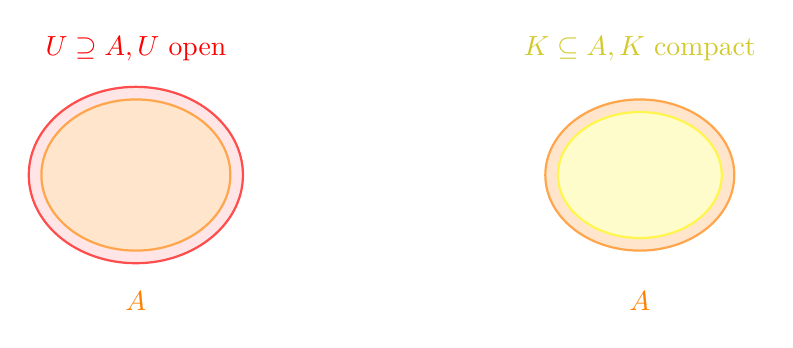
\begin{tikzpicture}[scale=0.8]
        \draw[thick, orange!70, fill=orange!20] (8, 0) ellipse (1.5 and 1.2) node {};
        % Draw the super set U
        \draw[thick, red!70, fill=red!10] (0, 0) ellipse (1.7 and 1.4) node {};
        % Draw the sub set K
        \draw[thick, yellow!70, fill=yellow!20] (8, 0) ellipse (1.3 and 1) node {};
        \draw[thick, orange!70, fill=orange!20] (0, 0) ellipse (1.5 and 1.2) node {};

        % Label the sets
        \node[orange] at (8, -2) {\(A\)};
        \node[orange] at (0, -2) {\(A\)};
        \node[red] at (0, 2) {\(U \supseteq A, U \text{ open}\)};
        \node[yellow!80!black] at (8, 2) {\(K \subseteq A, K \text{ compact}\)};
    \end{tikzpicture}
\end{center}

\subsubsection{Theorem: Heine-Borel}
On \(\mathbb{R}^n\), a set \(K\) is compact if and only if it is closed and bounded. In general, on a topological space, a set is compact if for any \(\{B_j\}_{j \in A}\) such that:
\[K \subset \bigcup_{j \in A} B_j,\]
there exists a finite subcover \(\{B_{j_1}, B_{j_2}, \ldots, B_{j_n}\}\) such that:
\[K \subset \bigcup_{i=1}^{n} B_{j_i}.\]

A measure \(\mu\) on a topological space with its Borel \(\sigma\)-algebra is called a \textit{Radon measure} if it is finite on compact sets and outer regular on Borel sets.

\subsubsection*{Observation}
The Lebesgue measure \(m\) on \(\mathbb{R}^n\) is a Radon measure. What are the other Radon measures on \(\mathbb{R}^n\)?

\subsubsection{Theorem: Characterization of Radon Measures on \(\mathbb{R}^n\)}
The Lebesgue measure \(m\) is the unique translation-invariant Radon measure on \(\mathbb{R}^n\) (up to a multiplicative constant).  
\begin{enumerate}
    \item \((\mathbb{R}^n, \mathcal{M}, m)\) is translation-invariant, i.e., for any \(A \in \mathcal{M}\) and any \(x \in \mathbb{R}^n\):
    \[m(A + x) = m(A),\]
    where \(A + x = \{a + x : a \in A\}\).
    \item If \(\mu : \mathcal{M} \to [0, \infty]\) is another translation-invariant Radon measure on \(\mathbb{R}^n\), then there exists a constant \(k > 0\) such that:
    \[\mu(A) = k \cdot m(A) \quad \text{for all } A \in \mathcal{M}.\]
\end{enumerate}

\subsection{Lebesgue-Stieltjes Measure}
Observe that a measure \(\mu\) on \(\mathcal{B}(\mathbb{R})\) satisfies:
\[\mu((-\infty, t]) \quad t \in \mathbb{R} \quad \text{is an increasing function and}\]
\[\mu((a, b]) = \mu((-\infty, b] \setminus (-\infty, a]) = \mu((-\infty, b]) - \mu((-\infty, a]) \quad \text{for } a < b.\]

We define \(g(t) = \mu((-\infty, t])\) for \(t \in \mathbb{R}\). Then \(g\) is an increasing function and we have the following theorem:
\subsubsection{Theorem: Lebesgue-Stieltjes Measure}
Let \(g: \mathbb{R} \to \mathbb{R}\) be an increasing function. Then, there exists a unique Radon measure \(\mu_g\) on \(\mathcal{B}(\mathbb{R})\) such that
\[\mu_g((a, b]) = g(b^+) - g(a^+) \quad \text{for all } a < b.\]
where:
\[g(t^+) = \lim_{x \to t^+} g(x) \quad \text{and} \quad g(t^-) = \lim_{x \to t^-} g(x).\]

The measure \(\mu_g\) is called the \textit{Lebesgue-Stieltjes measure} with \textit{distribution function} \(g\).

\subsubsection*{Observation}
If we consider \(g\) a right-continuous increasing function, then:
\[g(t^+) = \lim_{x \to t^+} g(x) = g(t).\]
Thus, in this case:
\[\mu_g((a, b]) = g(b) - g(a) \quad \text{for all } a < b.\]

\subsubsection*{Example}
Consider the function
\[g(x) = \begin{cases}
    x & \text{if } x < 0, \\
    2x + 1 & \text{if } 0 \leq x < 1, \\
    4 & \text{if } 1 \leq x \\
\end{cases}\]
Then, \(g\) is an increasing right-continuous function. Then, it defines a Lebesgue-Stieltjes measure \(\mu_g\). For example:
\[\mu_g((0, 2]) = g(2^+) - g(0^+) = 4 - 1 = 3.\]

\begin{center}
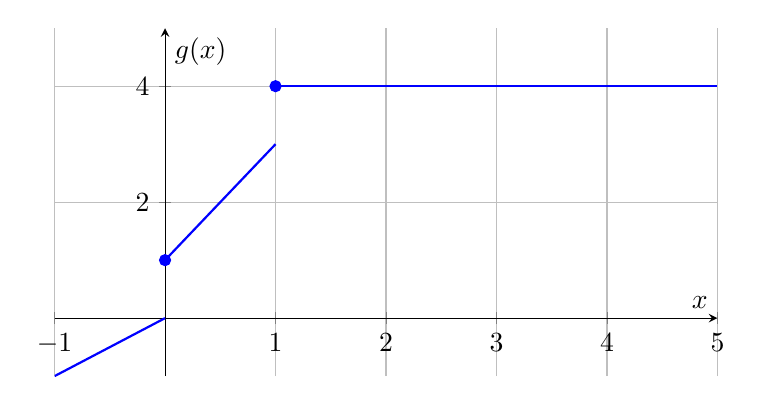
\begin{tikzpicture}[scale=1]
        \begin{axis}[
            axis lines = middle,
            xlabel = \(x\),
            ylabel = {\(g(x)\)},
            ymin = -1, ymax = 5,
            xmin = -1, xmax = 5,
            grid = both,
            width=10cm,
            height=6cm
        ]
        \addplot[
            domain=-1:0, 
            samples=100, 
            color=blue,
            thick
        ]{x};
        \addplot[
            domain=0:1, 
            samples=100, 
            color=blue,
            thick
        ]{2*x + 1};
        \addplot[
            domain=1:5, 
            samples=100, 
            color=blue,
            thick
        ]{4};
        % Add the jump at x=1
        \addplot[only marks, mark=*, color=blue] coordinates {(1,4)};
        \addplot[only marks, mark=*, color=blue] coordinates {(0,1)};
        \end{axis}
    \end{tikzpicture}
\end{center}

\subsubsection*{Observation}
If \(\mu\) is a Radon measure on \(\mathcal{B}(\mathbb{R})\), then there exists a unique increasing function \(g: \mathbb{R} \to \mathbb{R}\) such that \(\mu = \mu_g\).

\subsubsection{Properties of Lebesgue-Stieltjes Measure}
Let \(g: \mathbb{R} \to \mathbb{R}\) be an increasing function and \(\mu_g\) be the associated Lebesgue-Stieltjes measure. Then:
\begin{enumerate}[label=\alph*)]
    \item \(\mu_g\left(\{x\}\right) = g(x^+) - g(x^-)\) for all \(x \in \mathbb{R}\).
    \item \(g\) is continuous at \(x\) if and only if \(\mu_g(\{x\}) = 0\).
    \item \(\mu_g \left([a, b]\right) = g(b^+) - g(a^-)\) for all \(a < b\).
    \item \(\mu_g \left((a, b)\right) = g(b^-) - g(a^+)\) for all \(a < b\).
    \item \(\mu_g \left([a, b)\right) = g(b^-) - g(a^-)\) for all \(a < b\).
    \item If \(I \subset \mathbb{R}\) is an interval, then \(\mu_g(I) = 0\) if and only if \(g\) is constant on \(I\).
\end{enumerate}

\subsubsection*{Example}
Consider the function in the previous example:
\[g(x) = \begin{cases}
    x & \text{if } x < 0, \\
    2x + 1 & \text{if } 0 \leq x < 1, \\
    4 & \text{if } 1 \leq x \\
\end{cases}\]
Then, the associated Lebesgue-Stieltjes measure \(\mu_g\) satisfies:
\begin{itemize}
    \item \(\mu_g(\{0\}) = g(0^+) - g(0^-) = 1 - 0 = 1\).
    \item \(\mu_g(\{1\}) = g(1^+) - g(1^-) = 4 - 3 = 1\).
    \item \(\mu_g((0, 1)) = g(1^-) - g(0^+) = 3 - 1 = 2\).
    \item \(\mu_g([0, 1]) = g(1^+) - g(0^-) = 4 - 0 = 4\).
\end{itemize}

\section{Integration}
A \textit{simple function} on a measure space \((X, \mathcal{A}, \mu)\) is a \textit{measurable} function whose change consists of a finite number of values. Then, it is of the form:
\[s(x) = \sum_{j=1}^{n} c_j \chi_{A_j}(x),\]
where \(c_j \in [0, \infty)\), \(A_j \in \mathcal{A}\) for \(j = 1, 2, \ldots, n\), and \(\chi_{A_j}\) is the characteristic function of \(A_j\).

\subsubsection*{Example}
\[s(x) = \chi_{[a, b]} (x) \text{ is simple, and so is } s(x) = \chi_{\mathbb{Q}} (x).\]

\subsection{Theorem: Approximation of measurable functions}
For any measurable function \(f: X \to [0, \infty]\), there exists a sequence of simple functions \(\{s_n\}_{n=1}^{\infty}\) such that:
\begin{enumerate}
    \item \(0 \leq s_n(x) \leq s_{n+1}(x) \leq f(x)\) for all \(x \in X\).
    \item \(\lim_{n \to \infty} s_n(x) = f(x)\) for all \(x \in X\).
\end{enumerate}
\begin{proof}
For each \(n \in \mathbb{N}\), define the simple function \(s_n: X \to [0, \infty)\) by:
\[s_n(x) = \sum_{j=0}^{n2^n - 1} \frac{j}{2^n} \chi_{A_{j,n}}(x) + n \chi_{A_{n,n}}(x),\]
where:
\[A_{j,n} = \left\{x \in X : \frac{j}{2^n} \leq f(x) < \frac{j+1}{2^n}\right\} \text{ for } j = 0, 1, \ldots, n2^n - 1,\]
and
\[A_{n,n} = \{x \in X : f(x) \geq n\}.\]
Then, it is easy to verify that the sequence \(\{s_n\}_{n=1}^{\infty}\) satisfies the required properties.  
\end{proof}

\subsection{Integral of a simple function}
Let \(s: X \to [0, \infty)\) be a simple function of the form:
\[s(x) = \sum_{j=1}^{n} c_j \chi_{A_j}(x),\]
where \(c_j \in [0, \infty)\), \(A_j \in \mathcal{A}\) for \(j = 1, 2, \ldots, n\). Then, the integral of \(s\) with respect to the measure \(\mu\) is defined as:
\[\int_X s \,d\mu = \sum_{j=1}^{n} c_j \mu(A_j).\]

The itegral of a positive measurable function \(f: X \to [0, \infty]\) is defined as:
\[\int_X f \,d\mu = \sup\left\{\int_X s \,d\mu : 0 \leq s \leq f, s \text{ is simple}\right\}.\]

This integral is called the \textit{Lebesgue integral} of \(f\) with respect to the measure \(\mu\).

\subsubsection*{Example}
Consider the Dirichlet function of \(\mathbb{Q}\), defined as:
\[f(x) = \begin{cases}
    1 & \text{if } x \in \mathbb{Q}, \\
    0 & \text{if } x \notin \mathbb{Q}.
\end{cases}\]
Then, we can compute the Lebesgue integral of \(f\) with respect to the Lebesgue measure \(m\):
\[\int_{\mathbb{R}} \chi_{\mathbb{Q}} \,dm = m(\mathbb{Q})\cdot 1 + m(\mathbb{I}) \cdot 0 = 0.\]

\subsection{Properties of the Lebesgue Integral}
Let \(f, g: X \to [0, \infty]\) be measurable functions and \(A, B, E \in \mathcal{A}\). Then:
\begin{enumerate}
    \item \[ \int_E f \,d\mu = \int_X f \chi_E \,d\mu.\]
    \begin{proof}
        With \(f\) measurable, \(\exists\{s_n\}_{n = 1}^{\infty}\) simple functions such that \(s_n \nearrow f\). Consider \(f(x) \chi_E(x)\), then \(\{r_n(x) = s_n(x) \chi_E(x)\}_{n = 1}^{\infty}\) is a sequence of simple functions such that \(r_n \nearrow f \chi_E\). Thus:
        \[\int_X f \chi_E \,d\mu = \lim_{n \to \infty} \int_X r_n \,d\mu = \lim_{n \to \infty} \int_X s_n \chi_E \,d\mu = \lim_{n \to \infty} \int_E s_n \,d\mu = \int_E f \,d\mu.\]
    \end{proof}
    \item \[ \int_E (f + g) \,d\mu = \int_E f \,d\mu + \int_E g \,d\mu.\]
    \begin{proof}
        Let \(\{s_n\}_{n=1}^{\infty}\) and \(\{t_n\}_{n=1}^{\infty}\) be sequences of simple functions such that \(s_n \nearrow f\) and \(t_n \nearrow g\). Then, \(s_n + t_n \nearrow f + g\). Thus:
        \[\int_E (f + g) \,d\mu = \lim_{n \to \infty} \int_E (s_n + t_n) \,d\mu = \lim_{n \to \infty} \left(\int_E s_n \,d\mu + \int_E t_n \,d\mu\right) = \int_E f \,d\mu + \int_E g \,d\mu.\]
    \end{proof}
    \item \[\int_E \lambda f \,d\mu = \lambda \int_E f \,d\mu \quad \text{for any } \lambda \in \mathbb{R}.\]
    \item If \(f(x) \leq g(x)\) for all \(x \in E\), then:
    \[\int_E f \,d\mu \leq \int_E g \,d\mu.\]
    \item If \(A \subseteq B\), then:
    \[\int_A f \,d\mu \leq \int_B f \,d\mu.\]
    \item If \(f = 0\) almost everywhere on \(E\), that is, \(\mu(\{x \in E : f(x) \neq 0\}) = 0\), then:
    \[\int_E f \,d\mu = 0.\]
    \item If \(\mu(E) = 0\), then:
    \[\int_E f \,d\mu = 0.\]
    \item If \(A \cap B = \emptyset\), then:
    \[\int_{A \cup B} f \,d\mu = \int_A f \,d\mu + \int_B f \,d\mu.\]
    \item If \(f = g\) almost everywhere on \(X\), then:
    \[\int_X f \,d\mu = \int_X g \,d\mu.\]
\end{enumerate}

\subsection{General Functions}
Given a function \(f: X \to [-\infty, \infty]\), we can write it as:
\[f = f^+ - f^-,\]
where:
\[f^+(x) = \max\{f(x), 0\} \quad \text{and} \quad f^-(x) = \max\{-f(x), 0\}.\]
Both \(f^+\) and \(f^-\) are non-negative measurable functions.

\begin{center}
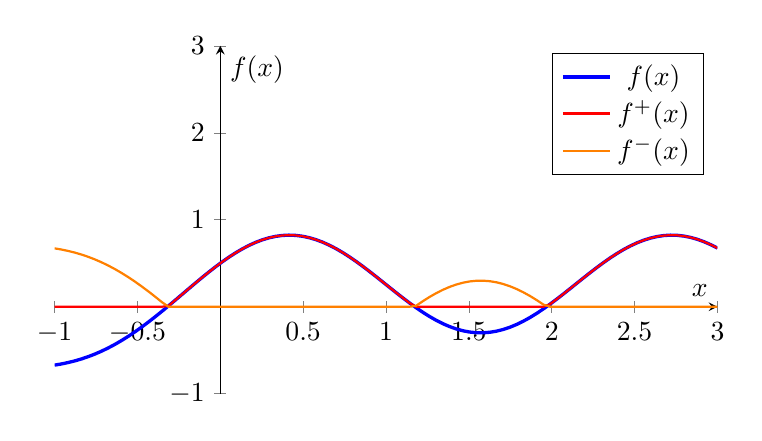
\begin{tikzpicture}[scale=1]
        \begin{axis}[
            axis lines = middle,
            xlabel = \(x\),
            ylabel = {\(f(x)\)},
            ymin = -1, ymax = 3,
            xmin = -1, xmax = 3,
            width=10cm,
            height=6cm
        ]
        \addplot[
            domain=-1:3, 
            samples=100, 
            color=blue,
            very thick
        ]{0.5*sin(deg(x)) + 0.5*cos(deg(2*x)) + 0.3*sin(deg(3*x))};
        % f^+
        \addplot[
            domain=-1:3, 
            samples=100, 
            color=red,
            thick
        ]{max(0, 0.5*sin(deg(x)) + 0.5*cos(deg(2*x)) + 0.3*sin(deg(3*x)))};
        % f^-
        \addplot[
            domain=-1:3, 
            samples=100, 
            color=orange,
            thick
        ]{max(0, -(0.5*sin(deg(x)) + 0.5*cos(deg(2*x)) + 0.3*sin(deg(3*x))))};
        % Add legend
        \legend{\(f(x)\), \(f^+(x)\), \(f^-(x)\)}
        \end{axis}
    \end{tikzpicture}
\end{center}

Then, we define the integral of \(f\) as:
\[\int_X f \,d\mu = \int_X f^+ \,d\mu - \int_X f^- \,d\mu,\]
provided that at least one of the integrals on the right-hand side is finite.

\subsection{Lebesgue Space}
On a measure space \((X, \mathcal{A}, \mu)\), the \textit{Lebesgue space} \(L^1(X, \mu)\) is defined as:
\[L^1(X, \mu) = \left\{f: X \to \mathbb{R} \text{ measurable} : \int_X |f| \,d\mu < \infty\right\}.\]
The elements of \(L^1(X, \mu)\) are equivalence classes, where two functions \(f\) and \(g\) are considered equivalent if they are equal almost everywhere, i.e., \(\mu(\{x \in X : f(x) \neq g(x)\}) = 0\). These functions are called \textit{Lebesgue-integrable functions}.

\subsubsection*{Example}
With the Lebesgue measure \(m\) on \(\mathbb{R}\), the function \(f(x) = \dfrac{1}{x^2}\) is in \(L^1([1, \infty], m)\), but not in \(L^1([0, 1], m)\).

\subsubsection*{Example}
On \(\mathbb{N}\), consider the counting measure \(\mu\) defined by \(\mu(A) = |A|\) for any \(A \subseteq \mathbb{N}\). Then, \(L^1(\mathbb{N}, \mu)\) is the space formed by functions \(f: \mathbb{N} \to \mathbb{R}\) such that:
\[\sum_{n=1}^{\infty} |f(n)| < \infty.\]

So \(f\) is such that the series \(\sum_{n=1}^{\infty} f(n)\) is absolutely convergent (i.e., convergent regardless of the order of its terms).

\subsubsection*{Example}
Now, consider again on \(\mathbb{N}\), the counting measure \(\mu\). Let \(f(x) = \dfrac{(-1)^n}{2^n}\). Then, \(f \in L^1(\mathbb{N}, \mu)\) since:
\[\int_{\mathbb{N}} |f| \,d\mu = \sum_{n=1}^{\infty} \left|\frac{(-1)^n}{2^n}\right| = \sum_{n=1}^{\infty} \frac{1}{2^n} = 1 < \infty.\]

\subsection{Corollary}
\(L^1(\mu)\) is a vector space, that is if \(f, g \in L^1(\mu)\) and \(\alpha, \beta \in \mathbb{R}\), then:
\[\alpha f + \beta g \in L^1(\mu), \quad \text{and} \quad \int_X (\alpha f + \beta g) \,d\mu = \alpha \int_X f \,d\mu + \beta \int_X g \,d\mu.\]

\subsubsection*{Remark}
If \(f \in L^1(\mu)\), then:
\[|f| \in L^1(\mu) \text{ and } \left|\int_X f \,d\mu\right| \leq \int_X |f| \,d\mu.\]

\subsection{Theorem: Monotone Convergence}
Consider a sequence of measurable functions \(\{f_n\}_{n=1}^{\infty}\) such that:
\begin{enumerate}
    \item \(0 \leq f_n(x) \leq f_{n+1}(x) \leq \infty\) for all \(x \in X\) and \(n \in \mathbb{N}\).
    \item \(\lim_{n \to \infty} f_n(x) = f(x)\) for all \(x \in X\).
\end{enumerate}
Then:
\[\int_X f(x) \,d\mu = \int_X \lim_{n \to \infty} f_n(x) \,d\mu = \lim_{n \to \infty} \int_X f_n(x) \,d\mu.\]

This integral may be infinite.

\subsubsection*{Example}
On \(X = [0, \infty]\), we define
\[f_n(x) = \begin{cases}
    1 - x^n & \text{if } 0 \leq x < 1, \\
    0 & \text{if } 1 \leq x 
\end{cases}\]
for \(n \in \mathbb{N}\). Then, 
\[0 \leq f_n(x) \leq f_{n+1}(x) \leq 1 \text{ for all } x \in [0, \infty]\]
and
\[\lim_{n \to \infty} f_n(x) = \begin{cases}
    1 & \text{if } 0 \leq x < 1, \\
    0 & \text{if } 1 \leq x 
\end{cases} = f(x).\]
Thus, by the Monotone Convergence Theorem:
\[\int_0^{\infty} f(x) \,dm = \int_0^{\infty} \lim_{n \to \infty} f_n(x) \,dm = \lim_{n \to \infty} \int_0^{\infty} f_n(x) \,dm.\]
Now, we compute:
\[\int_0^{\infty} f_n(x) \,dm = \int_0^1 (1 - x^n) \,dm = \left[x - \frac{x^{n+1}}{n+1}\right]_0^1 = 1 - \frac{1}{n+1} = \frac{n}{n+1}.\]
Thus:
\[\int_0^{\infty} f(x) \,dm = \lim_{n \to \infty} \frac{n}{n+1} = 1.\]  

\begin{center}
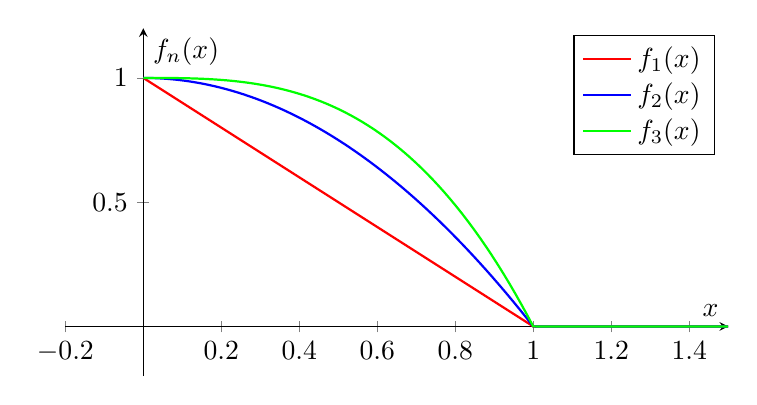
\begin{tikzpicture}[scale=1]
        \begin{axis}[
            axis lines = middle,
            xlabel = \(x\),
            ylabel = {\(f_n(x)\)},
            ymin = -0.2, ymax = 1.2,
            xmin = -0.2, xmax = 1.5,
            width=10cm,
            height=6cm
        ]
        % f_1
        \addplot[
            domain=0:1.5, 
            samples=100, 
            color=red,
            thick
        ]{max(1 - x, 0)};

        \addplot[
            domain=0:1.5, 
            samples=100, 
            color=blue,
            thick
        ]{max(1 - x^2, 0)};
        % f_3
        \addplot[
            domain=0:1.5, 
            samples=100, 
            color=green,
            thick
        ]{max(1 - x^3, 0)};
        % Add legend
        \legend{\(f_1(x)\),\(f_2(x)\),\(f_3(x)\)}
        \end{axis}
    \end{tikzpicture}
\end{center}

\subsubsection*{Example}
Now consider the sequence of functions
\[f_n(x) = \begin{cases}
    2^n & \text{if } 0 \leq x < \frac{1}{2^n}, \\
    0 & \text{if } \frac{1}{2^n} \leq x 
\end{cases}\]
for \(n \in \mathbb{N}\). Then,
\[0 \leq f_n(x) \leq f_{n+1}(x) \leq \infty \text{ for all } x \in [0, \infty]\]
and
\[\lim_{n \to \infty} f_n(x) = 0 \text{ for all } x \in [0, \infty].\]
Thus, by the Monotone Convergence Theorem:
\[\int_0^{\infty} f(x) \,dm = \int_0^{\infty} \lim_{n \to \infty} f_n(x) \,dm = \lim_{n \to \infty} \int_0^{\infty} f_n(x) \,dm.\]
Now, we compute:
\[\int_0^{\infty} f_n(x) \,dm = \int_0^{\frac{1}{2^n}} 2^n \,dm = 2^n \cdot \frac{1}{2^n} = 1.\]
Thus:
\[\int_0^{\infty} f(x) \,dm = \lim_{n \to \infty} 1 = 1.\]

\begin{center}
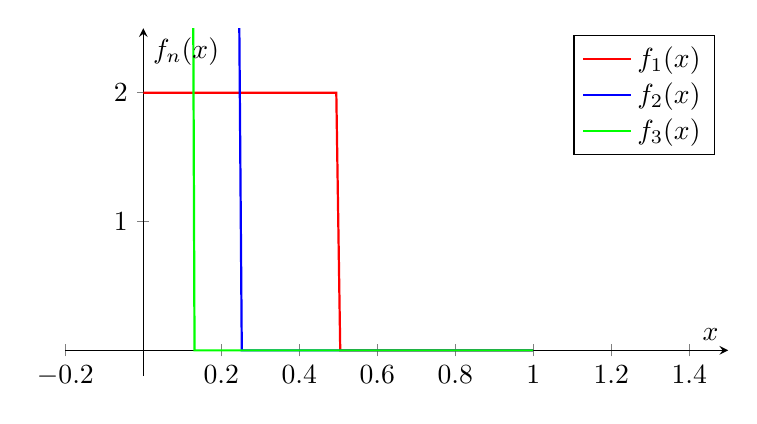
\begin{tikzpicture}[scale=1]
        \begin{axis}[
            axis lines = middle,
            xlabel = \(x\),
            ylabel = {\(f_n(x)\)},
            ymin = -0.2, ymax = 2.5,
            xmin = -0.2, xmax = 1.5,
            width=10cm,
            height=6cm
        ]
        % f_1
        \addplot[
            domain=0:1, 
            samples=100, 
            color=red,
            thick
        ]{(x < 0.5) * 2 + (x >= 0.5) * 0};
        % f_2
        \addplot[
            domain=0:1, 
            samples=100, 
            color=blue,
            thick
        ]{(x < 0.25) * 4 + (x >= 0.25) * 0};
        % f_3
        \addplot[
            domain=0:1, 
            samples=100, 
            color=green,
            thick
        ]{(x < 0.125) * 8 + (x >= 0.125) * 0};
        % Add legend
        \legend{\(f_1(x)\),\(f_2(x)\),\(f_3(x)\)}
        \end{axis}
    \end{tikzpicture}
\end{center}

\subsubsection{Proof of the Monotone Convergence Theorem}
We know that:
\[\left\{\int_X f_n(x) \,d\mu\right\}_{n=1}^{\infty}\]
is an increasing sequence, since \(f_n(x) \leq f_{n+1}(x)\) for all \(x \in X\). Thus, the limit:
\[\lim_{n \to \infty} \int_X f_n(x) \,d\mu\]
exists (possibly infinite). Also, since \(f_n(x) \leq f_{n+1}(x)\) for all \(x \in X\), we have:  
\[\int_X f_n(x) \,d\mu \leq \int_X f_{n+1}(x) \,d\mu \quad \text{for all } n \in \mathbb{N},\]
and 
\[\lim_{n \to \infty} \int_X f_n(x) \,d\mu \leq \int_X f(x) \,d\mu.\]

To prove the reverse inequality, consider an increasing sequence of simple functions approximating each \(f_n\):
\[r_{1,1}, r_{1,2}, \ldots, r_{1,k_1} \nearrow f_1,\]
\[r_{2,1}, r_{2,2}, \ldots, r_{2,k_2} \nearrow f_2,\]
\[\vdots\]
\[r_{n,1}, r_{n,2}, \ldots, r_{n,k_n} \nearrow f_n.\]
Define a new sequence of simple functions \(\{s_m\}_{m=1}^{\infty}\) as follows:
\[s_m = \max\{r_{n,k} : n, k \leq m\}.\]
Then, \(s_m \nearrow f\) as \(m \to \infty\). Thus:
\[\int_X f(x) \,d\mu = \lim_{m \to \infty} \int_X s_m(x) \,d\mu \leq \lim_{n \to \infty} \int_X f_n(x) \,d\mu. \qed\]

\subsection{Corollary}
For a sequence of positive measurable functions \(\{f_n\}_{n=1}^{\infty}\):
\[f(x) = \sum_{n=1}^{\infty} f_n(x) \quad \text{for all } x \in X,\]
we have:
\[\int_X f(x) \,d\mu = \sum_{n=1}^{\infty} \int_X f_n(x) \,d\mu.\]

\begin{proof}
Define the sequence of functions:
\[s_k(x) = \sum_{n=1}^{k} f_n(x) \quad \text{for } k \in \mathbb{N}.\]
Then, \(s_k(x) \nearrow f(x)\) as \(k \to \infty\). Thus, by the Monotone Convergence Theorem:
\[\int_X f(x) \,d\mu = \lim_{k \to \infty} \int_X s_k(x) \,d\mu = \lim_{k \to \infty} \sum_{n=1}^{k} \int_X f_n(x) \,d\mu = \sum_{n=1}^{\infty} \int_X f_n(x) \,d\mu. \qed\]
\end{proof}
\subsection{Fatou's Lemma}
Let \(\{f_n\}_{n=1}^{\infty}\) be a sequence of non-negative measurable functions on \(X\). Then:
\[\int_X \liminf_{n \to \infty} f_n(x) \,d\mu \leq \liminf_{n \to \infty} \int_X f_n(x) \,d\mu.\]
\begin{proof}
Define the sequence of functions:
\[g_n(x) = \inf_{k \geq n} f_k(x) \quad \text{for } n \in \mathbb{N}.\]
Then, \(g_n(x) \nearrow \liminf_{n \to \infty} f_n(x)\) as \(n \to \infty\). Thus, by the Monotone Convergence Theorem:
\[\int_X \liminf_{n \to \infty} f_n(x) \,d\mu = \lim_{n \to \infty} \int_X g_n(x) \,d\mu.\]
Also, since \(g_n(x) \leq f_n(x)\) for all \(x \in X\) and \(n \in \mathbb{N}\), we have:
\[\int_X g_n(x) \,d\mu \leq \int_X f_n(x) \,d\mu \quad \text{for all } n \in \mathbb{N}.\]
Thus:
\[\lim_{n \to \infty} \int_X g_n(x) \,d\mu \leq \liminf_{n \to \infty} \int_X f_n(x) \,d\mu. \qed\]
\end{proof}

\subsubsection*{Example}
Consider the sequence of functions:
\[f_n(x) = \begin{cases}
    \chi_{[0, 1]} (x) & \text{if } n \text{ is odd}, \\
    1 - \chi_{[0, 1]} (x) & \text{if } n \text{ is even}.
\end{cases}\]
Then, for all \(x \in \mathbb{R}\):
\[\liminf_{n \to \infty} f_n(x) = 0.\]
Thus:
\[\int_{\mathbb{R}} \liminf_{n \to \infty} f_n(x) \,dm = \int_{\mathbb{R}} 0 \,dm = 0.\]
On the other hand:
\[\int_{\mathbb{R}} f_n(x) \,dm = \begin{cases}
    1 & \text{if } n \text{ is odd}, \\
    \infty & \text{if } n \text{ is even}.
\end{cases}\]
Thus:
\[\liminf_{n \to \infty} \int_{\mathbb{R}} f_n(x) \,dm = 0.\]
Therefore, Fatou's Lemma holds:
\[\int_{\mathbb{R}} \liminf_{n \to \infty} f_n(x) \,dm = 0 \leq 0 = \liminf_{n \to \infty} \int_{\mathbb{R}} f_n(x) \,dm.\] 

\subsection{Theorem: Dominated Convergence}
Let \(\{f_n\}_{n=1}^{\infty}\) be a sequence of measurable functions on \(X\) such that:
\begin{enumerate}
    \item \(\lim_{n \to \infty} f_n(x) = f(x)\) for all \(x \in X\).
    \item There exists a function \(g \in L^1(X, \mu)\) such that \(|f_n(x)| \leq g(x)\) for all \(x \in X\) and \(n \in \mathbb{N}\).
\end{enumerate}
Then:
\[\int_X f(x) \,d\mu = \lim_{n \to \infty} \int_X f_n(x) \,d\mu, \quad f \in L^1(X, \mu) \quad \text{and} \quad \lim_{n \to \infty} \int_X |f_n(x) - f(x)| \,d\mu = 0.\]
\vskip 1em
\begin{proof}
Each \(f_n \in L^1(\mu)\), and so is \(f\), since:
\[|f(x)| = \lim_{n \to \infty} |f_n(x)| \leq g(x) \quad \text{for all } x \in X.\]
Also, since:
\[|f_n(x) - f(x)| \leq |f_n(x)| + |f(x)| \leq g(x) + g(x) = 2g(x) \quad \text{for all } x \in X,\]
we have:
\[2g(x) - |f_n(x) - f(x)| \geq 0 \quad \text{for all } x \in X.\]
Thus, by Fatou's Lemma:
\[\int_X \liminf_{n \to \infty} \left(2g(x) - |f_n(x) - f(x)|\right) \,d\mu \leq \liminf_{n \to \infty} \int_X \left(2g(x) - |f_n(x) - f(x)|\right) \,d\mu.\]
Now, since:
\[\liminf_{n \to \infty} \left(2g(x) - |f_n(x) - f(x)|\right) = \int_X 2g(x) - \limsup_{n \to \infty} |f_n(x) - f(x)| = 2g(x) - 0 = 2g(x),\]
we have:
\[\int_X 2g(x) \,d\mu \leq \liminf_{n \to \infty} \left(2\int_X g(x) \,d\mu - \int_X |f_n(x) - f(x)| \,d\mu\right).\]
Thus:
\[\limsup_{n \to \infty} \int_X |f_n(x) - f(x)| \,d\mu \leq 0.\]
Since the integral is non-negative, we conclude that:
\[\lim_{n \to \infty} \int_X |f_n(x) - f(x)| \,d\mu = 0.\]
Finally, by the triangle inequality:
\[\left|\int_X f_n(x) \,d\mu - \int_X f(x) \,d\mu\right| \leq \int_X |f_n(x) - f(x)| \,d\mu,\]
we have:
\[\lim_{n \to \infty} \left|\int_X f_n(x) \,d\mu - \int_X f(x) \,d\mu\right| = 0.\]
\end{proof}

\subsubsection*{Example}
Let us consider:
\[\lim_{n \to \infty} \int_0^1 \frac{\log(n + x)}{n} \cdot \sin(x) \,dx.\]
We have:
\[|f_n(x)| = \left|\frac{\log(n + x)}{n} \cdot \sin(x)\right| \leq \left|\frac{\log(n + x)}{n}\right| \leq 1 \in L^1([0, 1]).\]
So with \(g(x) = 1\), we can apply the Dominated Convergence Theorem:
\[\lim_{n \to \infty} \int_0^1 \frac{\log(n + x)}{n} \cdot \sin(x) \,dx = \int_0^1 \lim_{n \to \infty} \frac{\log(n + x)}{n} \cdot \sin(x) \,dx = \int_0^1 0 \cdot \sin(x) \,dx = 0.\]  

\subsection{Corollary: Uniform Convergence}
Let \(X, \mathcal{A}, \mu\) be a \underline{finite} measure space, that is, \(\mu(X) < \infty\). If a sequence of measurable functions \(\{f_n\}_{n=1}^{\infty}\) converges \underline{uniformly} to a function \(f\) on \(X\), then \(f \in L^1(X, \mu)\) and:
\[\lim_{n \to \infty} \int_X f_n(x) \,d\mu = \int_X f(x) \,d\mu.\]

\begin{proof}
The limit of \(f(x)\) satisfies:    
\[\inf_n |f_n(x)| \leq |f(x)| \leq \sup_n |f_n(x)| \quad \text{for all } x \in X.\]
Since \(f_n \in L^1(\mu)\), \(f\) is also integrable. Besides, by the uniform convergence:
\[\exists N \in \mathbb{N} : |f_n(x) - f(x)| < \epsilon \text{ for all } n \geq N \text{ and } x \in X.\]
Also:
\[|f_n(x)| \leq |f(x)| + \epsilon \implies \int_X |f_n(x)| \,d\mu \leq \int_X |f(x)| \,d\mu + \epsilon \mu(X) < \infty.\]
Thus, by the Dominated Convergence Theorem:
\[\lim_{n \to \infty} \int_X f_n(x) \,d\mu = \int_X f(x) \,d\mu.\]
\end{proof}

\subsection{Corollary}
Let \(X, \mathcal{A}, \mu\) be a measure space and \(f_n: X \to \mathbb{R}\) be a sequence of measurable functions such that:
\[\sum_{n=1}^{\infty} \int_X |f_n(x)| \,d\mu < \infty.\]
Then \(f \in L^1(X, \mu)\),
\[\sum_{n=1}^{\infty} f_n(x) \text{ converges to } f : X \to \mathbb{R},\]
and
\[\int_X f(x) \,d\mu = \sum_{n=1}^{\infty} \int_X f_n(x) \,d\mu.\]

\begin{proof}
Define:
\[g_N(x) = \sum_{n=1}^{N} f_n(x)\]
Then:
\[\int_X |g_N(x)| \,d\mu \leq \sum_{n=1}^{N} \int_X |f_n(x)| \,d\mu \leq \sum_{n=1}^{\infty} \int_X |f_n(x)| \,d\mu < \infty.\]
Thus, \(g_N \in L^1(X, \mu)\) for all \(N \in \mathbb{N}\). Now, 
\[\sum_{n=1}^{\infty} \int_X f_n(x) \,d\mu = \int_X \sum_{n=1}^{\infty} f_n(x) \,d\mu,\]
and finally:
\[\lim_{N \to \infty} \sum_{n=1}^{N} \int_X f_n(x) \,d\mu = \int_X \lim_{N \to \infty} g_N(x) \,dx.\]
\end{proof}

\section{Integration on Product Spaces}
Let \((X, \mathcal{A}, \mu)\) and \((Y, \mathcal{D}, \lambda)\) be two measure spaces. If
\[X \times Y = \{(x, y) : x \in X, y \in Y\},\]
we define the product \(\sigma\)-algebra \(\mathcal{A} \otimes \mathcal{D}\) as:
\[\mathcal{A} \otimes \mathcal{D} = \sigma (\mathcal{E}),\]
where:
\[\mathcal{E} = \{A \times D : A \in \mathcal{A}, D \in \mathcal{D}\}.\]

\subsection{Theorem: Product Measure}
There exists a unique measure \(\mu \otimes \lambda : \mathcal{A} \otimes \mathcal{D} \to [0, \infty]\) such that:
\[(\mu \otimes \lambda)(A \times D) = \mu(A) \cdot \lambda(D) \quad \text{for all } A \in \mathcal{A}, D \in \mathcal{D}.\]

\subsection{Product Measure Space}
The \textit{Product Measure Space} of \((X, \mathcal{A}, \mu)\) and \((Y, \mathcal{D}, \lambda)\) is the measure space:
\[(X \times Y, \mathcal{A} \otimes \mathcal{D}, \mu \otimes \lambda).\]

\subsubsection{Proposition}
The product measure space of the Lebesgue measure spaces \(\mathbb{R}^k\) and \(\mathbb{R}^{n-k}\) \((k < n)\), is the Lebesgue measure space \(\mathbb{R}^n\).

\subsubsection*{Observation}
We are going to consider in this section only \(\sigma\)-finite measure spaces.

\subsection{Sections of a Set}
If we consider a set \(E \subset X \times Y\), the \textit{sections} of \(E\) are defined as:
\[E_x = \{y \in Y : (x, y) \in E\} \quad \text{for } x \in X \quad \text{and} \quad E^y = \{x \in X : (x, y) \in E\} \quad \text{for } y \in Y.\]

\subsubsection{Sections of a Function}
If we consider a function \(f: X \times Y \to \overline{\mathbb{R}}\), the \textit{sections} of \(f\) are defined as:
\[f_x(y) = f(x, y) \quad \text{for } x \in X \quad \text{and} \quad f^y(x) = f(x, y) \quad \text{for } y \in Y.\]

\subsubsection{Proposition}
\begin{enumerate}
    \item If \(E \in \mathcal{A} \otimes \mathcal{D}\), then \(E_x \in \mathcal{D}\) for all \(x \in X\) and \(E^y \in \mathcal{A}\) for all \(y \in Y\).
    \item If \(f: X \times Y \to \overline{\mathbb{R}}\) is \(\mathcal{A} \otimes \mathcal{D}\)-measurable, then \(f_x: Y \to \overline{\mathbb{R}}\) is \(\mathcal{A} \otimes \mathcal{D}\)-measurable and \(f^y: X \to \overline{\mathbb{R}}\) is \(\mathcal{A} \otimes \mathcal{D}\)-measurable.
\end{enumerate}

\subsection{Cavalieri's Principle}
Let \(E \in \mathcal{A} \otimes \mathcal{D}\). Then:
\begin{enumerate}
    \item The function \(g(x) = \lambda(E_x)\) is \(\mathcal{A}\)-measurable and:
        \[\int_X g(x) \,d\mu = (\mu \otimes \lambda)(E).\]
    \item The function \(h(y) = \mu(E^y)\) is \(\mathcal{D}\)-measurable and:
        \[\int_Y h(y) \,d\lambda = (\mu \otimes \lambda)(E).\]
\end{enumerate}

\subsubsection*{Example}
Consider the set:
\[E = \{(x, y) : x \in [0, 2], y \in [x^3, x] \} \subset \mathbb{R} \times \mathbb{R}.\]
Then, 
\[m_x \otimes m_y (E) = \int_{[1, 2]} m_y(E_x) \,dm_x = \int_{[1, 2]} 2x \,dm_x = \left[x^2\right]_{1}^{2} = 4 - 1 = 3.\]

\subsection{Theorem: Fubini-Tonelli}
Let \(f: X \times Y \to [0, \infty]\) be a \underline{positive measurable} function. Then:
\begin{enumerate}
    \item The function \(F(x) = \int_Y f_x \,d\lambda\) is \(\mathcal{A}\)-measurable and:
        \[\int_{X} F(x) \,d\mu = \int_{X \times Y} f(x, y) \,d(\mu \otimes \lambda).\]
    \item The function \(G(y) = \int_X f^y \,d\mu\) is \(\mathcal{D}\)-measurable and:
        \[\int_{X \times Y} f(x, y) \,d(\mu \otimes \lambda) = \int_Y G(y) \,d\lambda.\]
\end{enumerate}

So we can integrate in the order we want.

\begin{proof}
For simple positive functions, Fubini-Tonelli's theorem is Cavalieri's Principle. Now, let \(f\) be a positive measurable function. Then, there exists an increasing sequence of simple functions \(\{s_n\}_{n=1}^{\infty}\) such that:
\[s_n(x, y) \nearrow f(x, y) \quad \text{for all } (x, y) \in X \times Y.\]
Thus, for each one of the simple functions \(s_n\):
\[\int_X \int_Y s_{n, x} \,d\lambda \,d\mu = \int_{X \times Y} s_n \,d(\mu \otimes \lambda) \]
and by the Monotone Convergence Theorem:
\[\int_X \left(\lim_{n \to \infty} \int_Y s_{n, x} \,d\lambda\right) d\mu = \lim_{n \to \infty} \int_{X \times Y} s_n \,d(\mu \otimes \lambda) = \int_{X \times Y} f(x, y) \,d(\mu \otimes \lambda).\]
Similarly, for \(f^y\), we have:
\[\int_Y \left(\lim_{n \to \infty} \int_X s_n^y \,d\mu\right) d\lambda = \lim_{n \to \infty} \int_{X \times Y} s_n \,d(\mu \otimes \lambda) = \int_{X \times Y} f(x, y) \,d(\mu \otimes \lambda).\]
So they are equal (Tonelli's theorem).

Now, if \(f \in L^1(X \times Y, \mu \otimes \lambda)\), we consider the positive and negative parts of \(f\):
\[f^+(x, y) = \max\{f(x, y), 0\},\]
\[f^-(x, y) = \max\{-f(x, y), 0\}.\]
Both \(f^+\) and \(f^-\) are positive measurable functions, and we can apply Tonelli's theorem to both of them.
\end{proof}

\subsubsection*{Example}
Consider \(X = Y = [0, 1]\), with \(\mu, \lambda\) being the Lebesgue measures. Consider the sequence:
\[0 < \delta_1 < \delta_2 < \ldots < \delta_n < 1\]
and define the continuous functions \(g_n\) with support in \((\delta_n, \delta_{n+1})\), i.e \(g_n(x) = 0\) for \(x \notin (\delta_n, \delta_{n+1})\), such that:
\[\int_0^1 g_n(x) \,dx = 1.\]
Now, define the function:
\[f(x, y) = \sum_{n=1}^{\infty} \left(g_n(x) - g_{n-1}(x)\right) g_n(y).\]
Observe that the support of each term is disjoint, only one term is non-zero for each \((x, y) \in [0, 1] \times [0, 1]\). Thus, \(f\) is well-defined and measurable. Now, we compute:
\[\int_0^1 \,dx \int_0^1 f(x, y) \,dy = \int_0^1 \,dx = 1.\]
On the other hand, we have:
\[\int_0^1 \,dy \int_0^1 f(x, y) \,dx = \int_0^1 0 \,dy = 0.\]
This happens because the integral of \(g_n(x) - g_{n-1}(x)\) with respect to the Lebesgue measure \(dx\) is zero for all \(n\).
In this case, \(f \notin L^1([0, 1] \times [0, 1])\), because:
\[\int_0^1 \,dx \int_0^1 |f(x, y)| \,dy = \infty.\]

\subsubsection*{Example}
Prove that:
\[e^{-x^2} \in L^1(\mathbb{R}),\]
and compute its integral.
\begin{center}
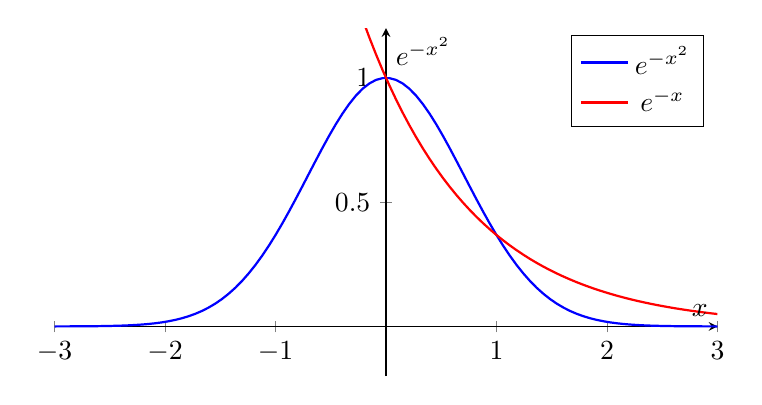
\begin{tikzpicture}[scale=1]
        \begin{axis}[
            axis lines = middle,
            xlabel = \(x\),
            ylabel = {\(e^{-x^2}\)},
            ymin = -0.2, ymax = 1.2,
            xmin = -3, xmax = 3,
            width=10cm,
            height=6cm
        ]
        % e^(-x^2)
        \addplot[
            domain=-3:3, 
            samples=100, 
            color=blue,
            thick
        ]{exp(-x^2)};
        \addplot[
            domain=-3:3, 
            samples=100, 
            color=red,
            thick,
        ]{exp(-x)};
        % Add legend
        \legend{\(e^{-x^2}\), \(e^{-x}\)}
        \end{axis}
    \end{tikzpicture}
\end{center}

\begin{proof}
On \([0, 1]\), \(e^{-x^2}\) is continuous and bounded, so 
\[\int_0^1 \left|e^{-x^2}\right| \,dx \leq \int_0^1 1 \,dx = 1 \implies e^{-x^2} \in L^1([0, 1]).\]
On \([1, \infty)\), we have:
\[0 < e^{-x^2} \leq e^{-x} \quad \text{ and } \quad \int_1^{\infty} e^{-x} \,dx = \lim_{N \to \infty} \int_1^{\infty} e^{-x} \chi_{[1, N]}(x) \,dx = \]
\[= \lim_{N \to \infty} \int_1^{N} e^{-x} \,dx = \lim_{N \to \infty} \left[-e^{-x}\right]_1^{N} = \lim_{N \to \infty} \left(-e^{-N} + e^{-1}\right) = e^{-1} < \infty \implies e^{-x} \in L^1([1, \infty)).\]
Thus, \(e^{-x^2} \in L^1([1, \infty)) \implies e^{-x^2} \in L^1([0, \infty))\).
Now, 
\[\int_{\mathbb{R}} e^{-x^2} \,dx = 2 \int_0^{\infty} e^{-x^2} \,dx. \implies e^{-x^2} \in L^1(\mathbb{R}).\]

To compute the integral, we consider:
\[I^2 = \left(\int_{\mathbb{R}} e^{-x^2} \,dx\right) \left(\int_{\mathbb{R}} e^{-y^2} \,dy\right) = \int_{\mathbb{R}} \int_{\mathbb{R}} e^{-(x^2 + y^2)} \,dx \,dy.\]
Now, we change to polar coordinates:
\[\int_0^{\infty} \int_0^{2\pi} e^{-r^2} r \,d\theta \,dr = 2\pi \int_0^{\infty} r e^{-r^2} \,dr = 2\pi \lim_{N \to \infty}\left[-\frac{e^{-r^2}}{2}\right]_0^{N} = \pi.\]
Thus:
\[\int_{\mathbb{R}} e^{-x^2} \,dx = \sqrt{\pi}.\]
\end{proof}

\subsection{Theorem: Fubini}
Let \(f: X \times Y \to \overline{\mathbb{R}}\) be an \underline{\(\mathcal{A} \otimes \mathcal{D}\)-measurable} function. Then, the integrals:
\[I_1 (f) = \int_{X \times Y} \left|f(x, y)\right| \,d\mu d\lambda,\]
\[I_2 (f) = \int_X \,d\mu \int_Y \left|f(x, y)\right| \,d\lambda,\]
\[I_3 (f) = \int_Y \,d\lambda \int_X \left|f(x, y)\right| \,d\mu.\]

exist and are equal (they can be finite or infinite). Besides, if they are finite, that is, if \(f \in L^1(X \times Y, \mu \otimes \lambda)\), then:
\[\int_{X \times Y} f(x, y) \,d(\mu \otimes \lambda) = \int_X \,d\mu \int_Y f(x, y) \,d\lambda = \int_Y \,d\lambda \int_X f(x, y) \,d\mu.\]

\subsubsection*{Observation}
The spaces \(X\) and \(Y\) must be \(\sigma\)-finite.



















































\end{document}
